\documentclass[a4paper, 12pt, oneside]{book}
\frenchspacing
\usepackage[warn]{mathtext}
\usepackage[utf8x]{inputenc}
\usepackage[english, russian]{babel}
\usepackage[T2A]{fontenc}
\usepackage{indentfirst}
\usepackage{misccorr}
\usepackage{ncccomma}
\usepackage{amsmath}
\usepackage{graphicx}
\usepackage{paralist}
\usepackage{topcapt}
\usepackage[section]{placeins}
\usepackage{graphicx}
\usepackage[usenames]{color}
\usepackage{colortbl}
\usepackage{longtable}
\usepackage{multirow}
\usepackage{enumitem}
\usepackage{listings}
\usepackage[unicode=true, hidelinks=true]{hyperref}
\renewcommand{\phi}{\varphi}
\renewcommand{\le}{\leqslant}
\renewcommand{\ge}{\geqslant}
\renewcommand{\kappa}{\varkappa}
\renewcommand{\epsilon}{\varepsilon}
%Все эти математические пакеты, по большому счёту, не нужны, просто один шаблон использую для документов, чтобы ничего не забыть
\begin{document}
 \tableofcontents
 \newpage 
 \hypersetup{hidelinks=false}
 \pagestyle{headings}
 \part{Компьютерная грамотность}\label{base}
\chapter{Введение}
Введение.
\section{Тонны матана}
\chapter{Операционная система}\label{base:os}
\section{История}\label{base:os:history}
Операционные системы (ОС) предоставляют набор функциональности, необходимой для работы большинства приложений на компьютере, а также связующие механизмы для контроля и синхронизации. На первых компьютерах не было операционных систем, поэтому каждая исполняемая программа должна была знать полную аппаратную спецификацию машины и выполнять стандартные задачи, а также иметь собственные драйверы для периферийных устройств, таких как принтеры и кардридеры. Возрастающая сложность оборудования и пользовательских программ привела к появлению операционных систем.

\subsection{Предыстория}\label{base:os:history:prehistory}
Раньше пользователь получал машину в единоличное пользование; он приходил с программой и данными, обычно записанными на перфокартах или магнитных лентах. Программа загружалась в машину, которая начинала работать, до тех пор пока программа не завершалась или не выдавала ошибку. Отладка программ осуществлялась при помощи панели управления, снабжённой тумблерами и лампочками. Наибольших успехов в этом достиг Алан Тьюринг на ранней машине Манчестерский Марк I, к тому времени он уже разрабатывал основные принципы работы операционных систем.

Более поздние машины имели библиотеки, которые связывались с пользовательской программой для поддержки таких операций как ввод и вывод. Это было началом современных операционных систем. Однако машины всё ещё выполняли одну задачу за один промежуток времени.

По мере увеличения производительности машин, время на исполнение программ уменьшалось, а время передачи оборудования от одного пользователя другому оставалось прежним. Выстраивались длинные очереди из людей, желающих запустить свою программу, каждый из них имел по несколько магнитных лент с программами и данными. Операторы машин не успевали контролировать все операции, проводимые с компьютерами, поэтому возникла необходимость в автоматическом контроле и выявлении ошибок.

Эти требования были учтены при создании первых операционных систем. Сначала для этого были использованы библиотеки времени исполнения, которые запускались до первой пользовательской задачи, считывали информацию с носителей, контролировали исполнение, записывали результаты и немедленно переключались на исполнение следующей задачи.

\subsection{Эра мейнфреймов}\label{base:os:history:mainframe}
Первой в мире операционной системой считается GM OS (General Motors Operating System).
Ранние операционные системы были очень разнородными, каждый поставщик или заказчик создавали одну или более систем для конкретного компьютера. Каждая операционная система, даже одного производителя, могла иметь совершенно разные команды и возможности. Обычно с появлением новой машины появлялась и новая операционная система, и приложения приходилось приспосабливать, перекомпилировать и перепроверять.

\subsubsection{Системы для оборудования IBM}\label{base:os:history:ibm}
Такое состояние дел продолжалось до 1960-х, когда IBM, лидирующий поставщик оборудования на тот момент, прекратила разработку существующих систем и направила усилия на создание серии машин System/360, все представители которой должны были использовать одинаковые инструкции и архитектуру ввода/вывода. IBM начала разрабатывать единую операционную систему для этих машин, OS/360. Проблемы, возникшие при создании OS/360, стали легендарными и были описаны в книге <<Мифический человеко-месяц>> Фредерика Брукса. Из-за различий в производительности и задержек при разработке программного обеспечения, вместо единой OS/360 было представлено семейство операционных систем под таким же названием.

IBM выпустила ещё несколько операционных систем, среди них три оказались наиболее долгоживущими:
\begin{itemize}
 \item \textbf{OS/MFT} для систем среднего класса. Она имела одного преемника, систему OS/VSI, развитие которой продолжалось до 1980-х.
 \item \textbf{OS/MVT} для крупных машин. Она была сходна с OS/MFT (программы могли переноситься между ними без перекомпилирования), но имела более продвинутое управление памятью и систему разделения времени, TSO. MVT имела несколько наследников, включая z/OS.
 \item \textbf{DOS/360} для низших моделей System/360 имела несколько преемников, включая z/VSE, используемую до настоящего времени. Она значительно отличалась от OS/MFT и OS/MVT.
\end{itemize}

IBM поддерживает полную совместимость, поэтому разработанные в шестидесятых программы всё ещё можно запускать под z/VSE (если они создавались для DOS/360) или z/OS (если создавались для OS/MFT или OS/MVT) без изменений.

IBM разрабатывала, но официально не выпустила TSS/360, операционную сиcтему с разделением времени для S/360 Model 67.

Несколько операционных систем для архитектур IBM S/360 и S/370 были разработаны третьими фирмами, включая \selectlanguage{english}Michigan Terminal System (MTS)\selectlanguage{russian} и MUSIC/SP.

\subsubsection{Другие операционные системы для мейнфреймов}\label{base:os:history:other}
Control Data Corporation разработала операционную систему SCO\-PE в 1960-х для обработки пакетных заданий. В сотрудничестве с Университетом Миннесота были созданы операционные системы KRONOS и NOS в 1970-х, которые поддерживали одновременный запуск заданий и разделение времени.

В конце 1970-х Control Data и Университет Иллинойс разработали машину PLATO, привнесшей множество инноваций для своего времени. Система использовала язык программирования TUTOR, что позволило создавать такие программы, как чат в реальном времени и многопользовательские графические игры.

UNIVAC, первый производитель коммерческих компьютеров, создала серию операционных систем EXEC. Как большинство ранних операционных систем для мейнфреймов, это были операционные системы, ориентированные на обработку пакетных заданий. В 1970-х UNIVAC выпустила систему Real-Time Basic.

Burroughs Corporation представила машину B5000 в 1961 с операционной системой MCP (Master Control Program). B5000 поддерживала исключительно языки высокого уровня и не поддерживала машинные языки или ассемблер; таким образом, MCP стала первой операционной системой, написанной только на высокоуровневом языке (ESPOL, диалект Алгола). MCP также представила несколько инноваций, включая первую коммерческую реализацию виртуальной памяти. MCP по сей день используется на компьютерах Unisys ClearPath/MCP.

Project MAC разработал Multics и \selectlanguage{english} General Electric Comprehensive Operating Supervisor (GECOS), \selectlanguage{russian} в которых была введена концепция уровней привилегий.

Digital Equipment Corporation разработала множество операционных систем для своих различных линеек компьютеров, включая TOPS-10 и TOPS-20 с разделением времени для 36-битных машин PDP-10. До широкого рапространения UNIX, TOPS-10 пользовалась большой популярностью в университетах и раннем сообществе ARPANET.

\subsection{Миникомпьютеры и развитие UNIX}\label{base:os:history:unix}
Начальные версии операционной системы UNIX были разработаны в AT\&T Bell Laboratories в конце 1960-х. Будучи абсолютно бесплатной в первых версиях и легко модифицируемой, эта система завоевала большую популярность. Так как UNIX была написана на языке высокого уровня Си, её можно легко было перенести на новую аппаратную архитектуру. Эта переносимость позволила ей стать основной системой для второго поколения миникомпьютеров и первого поколения рабочих станций.

В то же время Digital Equipment Corporation создала простую операционную систему RT-11 для серии 16 битных машин PDP-11, и систему VMS для 32-битных компьютеров VAX.

Другой разработкой этого времени стала операционная система Pick от Microdata Corporation.

\section{Классификация}\label{base:os:classification}
\subsection{История}\label{base:os:classification:history}
\subsection{Пользователи}\label{base:os:classification:users}
\subsection{Задачи}\label{base:os:classification:tasks}
\section{Структура операционной системы}
\emph{Операционная система} --- сложный комплекс разнообразных программ, с одной стороны являющихся интерфейсом между устройствами вычислительной системы и прикладными программами, а с другой --- предназначенных для управления устройствами, управления вычислительными процессами, эффективного распределения вычислительных ресурсов между вычислительными процессами и организации надёжных вычислений.


\subsection{Ядро}
Ядро --- центральная часть операционной системы (ОС), обеспечивающая приложениям координированный доступ к ресурсам компьютера, таким как процессорное время, память, внешнее аппаратное обеспечение, внешнее устройство ввода и вывода информации. Также обычно ядро предоставляет сервисы файловой системы и сетевых протоколов.

Как основополагающий элемент ОС, ядро представляет собой наиболее низкий уровень абстракции для доступа приложений к ресурсам системы, необходимым для их работы. Как правило, ядро предоставляет такой доступ исполняемым процессам соответствующих приложений за счёт использования механизмов межпроцессного взаимодействия и обращения приложений к системным вызовам ОС.

Описанная задача может различаться в зависимости от типа архитектуры ядра и способа её реализации.

\subsubsection{Типы архитектур ядер операционных систем}
\paragraph{Монолитное.} Классическая и, на сегодняшний день, наиболее распространённая архитектура ядер операционных систем --- это \emph{монолитные} ядра. Они предоставляют богатый набор абстракций оборудования. Все части монолитного ядра работают в одном адресном пространстве.

Монолитные ядра имеют долгую историю развития и усовершенствования и, на данный момент, являются наиболее архитектурно зрелыми и пригодными к эксплуатации. Вместе с тем, монолитность ядер усложняет их отладку, понимание кода ядра, добавление новых функций и возможностей, удаление <<мёртвого>>, ненужного, унаследованного от предыдущих версий кода. <<Разбухание>> кода монолитных ядер также повышает требования к объёму оперативной памяти, требуемому для функционирования ядра ОС. Это делает монолитные ядерные архитектуры малопригодными к эксплуатации в системах, сильно ограниченных по объёму ОЗУ, например, встраиваемых системах, производственных микроконтроллерах и~т.\,д..

\paragraph{Модульное.} Ограниченность и громоздкость монолитных ядер привели к появлению т.\,н.~\emph{модульных} ядер.

В отличие от <<классических>> монолитных ядер, считающихся ныне устаревшими, модульные ядра, как правило, не требуют полной перекомпиляции ядра при изменении состава аппаратного обеспечения компьютера. Вместо этого модульные ядра предоставляют тот или иной механизм подгрузки модулей ядра, поддерживающих то или иное аппаратное обеспечение (например, драйверов). При этом подгрузка модулей может быть как динамической (выполняемой <<на лету>>, без перезагрузки ОС, в работающей системе), так и статической (выполняемой при перезагрузке ОС после переконфигурирования системы на загрузку тех или иных модулей).

Все модули ядра работают в адресном пространстве ядра и могут пользоваться всеми функциями, предоставляемыми ядром. Поэтому модульные ядра продолжают оставаться монолитными. Модульность ядра осуществляется на уровне бинарного образа, а не на архитектурном уровне ядра, так как динамически подгружаемые модули загружаются в адресное пространство ядра и в дальнейшем работают как интегральная часть ядра. Модульные монолитные ядра не следует путать с архитектурным уровнем модульности, присущий микроядрам и гибридным ядрам. Практически, динамичная загрузка модулей, это просто более гибкий способ изменения образа ядра во время выполнения — в отличие от перезагрузки с другим ядром. Модули позволяют легко расширить возможности ядра по мере необходимости.

Модульные ядра удобнее для разработки, чем традиционные монолитные ядра, не поддерживающие динамическую загрузку модулей, так как от разработчика не требуется многократная полная перекомпиляция ядра при работе над какой-либо его подсистемой или драйвером. Выявление, локализация, отладка и устранение ошибок при тестировании также облегчаются.

Модульные ядра предоставляют особый программный интерфейс (API) для связывания модулей с ядром, для обеспечения динамической подгрузки и выгрузки модулей. В свою очередь, не любая программа может быть сделана модулем ядра: на модули ядра накладываются определённые ограничения в части используемых функций (например, они не могут пользоваться функциями стандартной библиотеки С/С++ и должны использовать специальные аналоги, являющиеся функциями API ядра). Кроме того, модули ядра обязаны экспортировать определённые функции, нужные ядру для правильного подключения и распознавания модуля, для его корректной инициализации при загрузке и корректного завершения при выгрузке, для регистрации модуля в таблице модулей ядра и для обращения из ядра к сервисам, предоставляемым модулем.

Не все части ядра могут быть сделаны модулями. Некоторые части ядра всегда обязаны присутствовать в оперативной памяти и должны быть жёстко <<вшиты>> в ядро. Также не все модули допускают динамическую подгрузку (без перезагрузки ОС). Общей тенденцией развития современных модульных ядер является всё большая модуляризация кода, улучшение механизмов динамической подгрузки и выгрузки, уменьшение или устранение необходимости в ручной подгрузке модулей или в переконфигурации ядра при изменениях аппаратуры путём введения тех или иных механизмов автоматического определения оборудования и автоматической подгрузки нужных модулей, универсализация кода ядра и введение в ядро абстрактных механизмов, предназначенных для совместного использования многими модулями. Примером может служить VFS --- <<виртуальная файловая система>>, совместно используемая многими модулями файловых систем в ядре Linux.

\paragraph{Микроядро.} \emph{Микроядро} --- это минимальная реализация функций ядра операционной системы.

Классические микроядра предоставляют лишь очень небольшой набор низкоуровневых примитивов, или системных вызовов, реализующих базовые сервисы операционной системы.

К ним относятся:
\begin{itemize}
 \item управление адресным пространством оперативной памяти.
 \item управление адресным пространством виртуальной памяти.
 \item управление процессами и потоками (нитями).
 \item средства межпроцессной коммуникации.
\end{itemize}

Все остальные сервисы ОС, в классических монолитных ядрах предоставляемые непосредственно ядром, в микроядерных архитектурах реализуются в адресном пространстве пользователя (Ring3) и называются сервисами. Примерами таких сервисов, выносимых в пространство пользователя в микроядерных архитектурах, являются сетевые сервисы, файловая система, драйверы.

Основное достоинство микроядерной архитектуры --- высокая степень модульности ядра операционной системы. Это существенно упрощает добавление в него новых компонентов. В микроядерной операционной системе можно, не прерывая её работы, загружать и выгружать новые драйверы, файловые системы и т. д. Существенно упрощается процесс отладки компонентов ядра, так как новая версия драйвера может загружаться без перезапуска всей операционной системы. Компоненты ядра операционной системы ничем принципиально не отличаются от пользовательских программ, поэтому для их отладки можно применять обычные средства. Микроядерная архитектура повышает надежность системы, поскольку ошибка на уровне непривилегированной программы менее опасна, чем отказ на уровне режима ядра. И чтобы добавить в ОС с микроядром драйвер того или иного устройства, не надо перекомпилировать всё ядро, а надо лишь отдельно откомпилировать этот драйвер и запустить его в пользовательском пространстве.

В то же время микроядерная архитектура операционной системы вносит дополнительные накладные расходы, связанные с обменом сообщениями, что отрицательно влияет на производительность. Для того чтобы микроядерная операционная система по скорости не уступала операционным системам на базе монолитного ядра, требуется очень аккуратно проектировать разбиение системы на компоненты, стараясь минимизировать взаимодействие между ними. Таким образом, основная сложность при создании микроядерных операционных систем --- необходимость очень аккуратного проектирования.

Микроядра типа ядра ОС Minix и GNU Hurd развиваются медленно, гораздо медленнее, чем Linux и ядро систем семейства BSD. По словам создателя Minix3, Таненбаума, он пытается <<построить сверхнадёжную систему. Она может использоваться в том числе на серверах, которым необходимы годы безотказной работы>>.

Классическим примером микроядерной системы является Symbian OS. Это пример распространенной и отработанной микроядерной (a начиная c версии Symbian OS v8.1, и наноядерной) операционной системы. Создателям Symbian OS удалось совместить эффективность и концептуальную стройность, несмотря на то что современные версии этой системы предоставляют обширные возможности, в том числе средства для работы c потоковыми данными, стеками протоколов, критичными к латентности ядра, графикой и видео высокого разрешения). Разработчики Symbian вынесли практически все прикладные (т.e. выходящие за пределы компетенции ядра) задачи в модули-серверы, функционирующие в пользовательском адресном пространстве.

В ОС Windows NT версий 3.х микроядерная архитектура с сервисным процессом использовалась для подсистемы графики и пользовательского интерфейса. В частности, драйвер графической аппаратуры загружался в контекст сервисного процесса, а не ядра. Начиная с версии 4, от этого отказались, сервисный процесс сохранился только для управления консольными окнами командной строки, а собственно графическая подсистема вместе с драйвером аппаратуры (в том числе трехмерной графики) переместилась в специально обособленный регион ядра ОС.

ОС Windows CE (и созданные на её основе сборки, такие, как Windows Mobile), будучи практически полностью совместимой (как подмножество) с Windows NT по вызовам и методам программирования приложений, тем не менее полностью отличается от Windows NT по внутренней архитектуре и является микроядерной ОС с выносом всех драйверов устройств, сетевых стеков и графической подсистемы в сервисные процессы.

Недостаток --- плата за принудительное «переключение» процессов в ядре (переключение контекста); этот факт собственно и объясняет трудности в проектировании и написании ядер подобной конструкции. Эти недостатки способны обойти ОС, использующие архитектуру экзоядра, являющуюся дальнейшим развитием микроядерной архитектуры.

\paragraph{Экзоядро.} В традиционных операционных системах ядро предоставляет не только минимальный набор сервисов, обеспечивающих выполнение программ, но и большое количество высокоуровневых абстракций для использования разнородных ресурсов компьютера: оперативной памяти, жестких дисков, сетевых подключений. В отличие от них, ОС на основе \emph{экзоядра} предоставляет лишь набор сервисов для взаимодействия между приложениями, а также необходимый минимум функций, связанных с защитой: выделение и высвобождение ресурсов, контроль прав доступа, и~т.\,д. Экзоядро не занимается предоставлением абстракций для физических ресурсов --- эти функции выносятся в библиотеку пользовательского уровня (так называемую libOS).

Основная идея операционной системы на основе экзоядра состоит в том, что ядро должно выполнять лишь функции координатора для небольших процессов, связанных только одним ограничением --- экзоядро должно иметь возможность гарантировать безопасное выделение и освобождение ресурсов оборудования. В отличие от ОС на основе микроядра, ОС, базирующиеся на экзоядре, обеспечивают гораздо большую эффективность за счет отсутствия необходимости в переключении между процессами при каждом обращении к оборудованию.

Архитектуры на основе экзоядер являются дальнейшим развитием и усовершенствованием микроядерных архитектур и одновременно ужесточают требования к минималистичности и простоте кода ядра. libOS может обеспечивать произвольный набор абстракций, совместимый с той или иной уже существующей операционной системой, например GNU/Linux или Windows.

\paragraph{Наноядро.} \emph{Наноядро} --- архитектура ядра операционной системы компьютеров, в рамках которой крайне упрощённое и минималистичное ядро выполняет лишь одну задачу --- обработку аппаратных прерываний, генерируемых устройствами компьютера. После обработки прерываний от аппаратуры наноядро, в свою очередь, посылает информацию о результатах обработки (например, полученные с клавиатуры символы) вышележащему программному обеспечению при помощи того же механизма прерываний. Также часто реализуют минимальную поддержку потоков:~создание и переключение.

В некотором смысле концепция наноядра близка к концепции HAL --- Hardware Abstraction Layer, предоставляя вышележащему ПО удобные механизмы абстракции от конкретных устройств и способов обработки их прерываний.

Наиболее часто в современных компьютерах наноядра используются для виртуализации аппаратного обеспечения реальных компьютеров или для реализации механизма гипервизора, с целью позволить нескольким или многим различным операционным системам работать одновременно и параллельно на одном и том же компьютере. Например, VMware ESX Server реализует собственное наноядро, не зависимое от ОС и устанавливаемое на <<голое железо>>. Поверх этого наноядра работают пользовательские и административные утилиты VMware и сами операционные системы, виртуализируемые в ESX Server.

Наноядра также могут использоваться для обеспечения переносимости (портабельности) операционных систем на разное аппаратное обеспечение или для обеспечения возможности запуска <<старой>> операционной системы на новом, несовместимом аппаратном обеспечении без её полного переписывания и портирования. Например, фирма Apple Computer использовала наноядро в версии Mac OS Classic для PowerPC для того, чтобы транслировать аппаратные прерывания, генерировавшиеся их компьютерами на базе процессоров PowerPC в форму, которая могла <<пониматься>> и распознаваться Mac OS для процессоров Motorola 680x0. Таким образом, наноядро эмулировало для Mac OS <<старое>> 680x0 железо. Альтернативой было бы полное переписывание и портирование кода Mac OS на PowerPC при переходе с 680x0 на них. Позднее, в эпоху Mac OS 8.6, наноядро виртуализировало предоставляемые PowerPC мультипроцессорные возможности и обеспечивало поддержку SMP в Mac OS. Другие удачные примеры использования наноядерных архитектур включают наноядро Adeos, работающее как модуль ядра для Linux и позволяющее выполнять одновременно с Linux какую-либо операционную систему реального времени.

Наноядро может быть настолько маленьким и примитивным, что даже важнейшие устройства, находящиеся непосредственно на материнской плате или на плате контроллера встраиваемого устройства, такие, как таймер или программируемый контроллер прерываний, обслуживаются специальными драйверами устройств, а не непосредственно ядром. Такого рода сверхминималистичные наноядра называют иногда пикоядрами.

Термин <<наноядро>> иногда неформально используется для описания очень маленьких, упрощённых и лёгких микроядер, таких, как L4.

\paragraph{Гибридное ядро.} \emph{Гибридное ядро} --- модифицированные микроядра (минимальная реализация основных функций ядра операционной системы компьютера), позволяющие для ускорения работы запускать <<несущественные>> части в пространстве ядра.

Все рассмотренные подходы к построению операционных систем имеют свои достоинства и недостатки. В большинстве случаев современные операционные системы используют различные комбинации этих подходов. Так, например сейчас, Linux представляет собой монолитную систему с отдельными элементами модульного ядра. При компиляции ядра можно разрешить динамическую загрузку и выгрузку очень многих компонентов ядра --- так называемых модулей. В момент загрузки модуля его код загружается на уровне системы и связывается с остальной частью ядра. Внутри модуля могут использоваться любые экспортируемые ядром функции.

Существуют варианты ОС GNU (Debian GNU/Hurd), в которых вместо монолитного ядра применяется ядро Mach (такое же, как в Hurd), а поверх него в пользовательском пространстве работают те же самые процессы, которые при использовании Linux были бы частью ядра. Другим примером смешанного подхода может служить возможность запуска операционной системы с монолитным ядром под управлением микроядра. Так устроены 4.4BSD и MkLinux, основанные на микроядре Mach. Микроядро обеспечивает управление виртуальной памятью и работу низкоуровневых драйверов. Все остальные функции, в том числе взаимодействие с прикладными программами, осуществляется монолитным ядром. Данный подход сформировался в результате попыток использовать преимущества микроядерной архитектуры, сохраняя по возможности хорошо отлаженный код монолитного ядра.

Наиболее тесно элементы микроядерной архитектуры и элементы монолитного ядра переплетены в ядре Windows NT. Хотя Windows NT часто называют микроядерной операционной системой, это не совсем так. Микроядро NT слишком велико (более 1 Мбайт, кроме того, в ядре системы находится, например, ещё и модуль графического интерфейса), чтобы носить приставку <<микро>>. Компоненты ядра Windows NT располагаются в вытесняемой памяти и взаимодействуют друг с другом путем передачи сообщений, как и положено в микроядерных операционных системах. В то же время все компоненты ядра работают в одном адресном пространстве и активно используют общие структуры данных, что свойственно операционным системам с монолитным ядром. Причина проста: чисто микроядерный дизайн коммерчески менее выгоден, поскольку менее эффективен (за счет накладных расходов на передачу сообщений там, где можно было обойтись вызовами функций).Таким образом, Windows NT можно с полным правом назвать гибридной операционной системой.

Смешанное ядро, в принципе, должно объединять преимущества монолитного ядра и микроядра: казалось бы, микроядро и монолитное ядро --- крайности, а смешанное --- золотая середина. В них возможно добавлять драйвера устройств двумя способами: и внутрь ядра, и в пользовательское пространство. Но на практике концепция смешанного ядра часто подчёркивает не только достоинства, но и недостатки обоих типов ядер.

\paragraph{Сравнение ядер различных типов.}
Приведём таблицу сравнения различных архитектурных типов:
\newcolumntype{G}{>{\columncolor[rgb]{0, 1, 0}}c}
\newcolumntype{g}{>{\columncolor[rgb]{0.8, 1, 0.8}}p{4cm}}
\newcolumntype{B}{>{\columncolor[rgb]{1, 0, 0}}c}
\newcolumntype{b}{>{\columncolor[rgb]{1, 0.8, 0.8}}p{4cm}}
\def\tabrowsep{\noalign{\vskip 2pt}}
\begin{longtable}{lgb}
 Тип                         & \multicolumn{1}{G}{Достоинства} & \multicolumn{1}{B}{Недостатки} \\ \tabrowsep
 Монолитное & Скорость работы, упрощённая разработка модулей & Поскольку всё ядро работает в одном адресном пространстве, сбой в одном из компонентов может нарушить работоспособность всей системы, громоздкость \\ \tabrowsep
 Модульное & Те же, что у монолитного + большая гибкость & Те же, что у монолитного \\ \tabrowsep
 Микроядро & Устойчивость к сбоям оборудования, ошибкам в компонентах системы, упрощённое добавление новых компонентов и их отладки. & Передача данных между процессами требует накладных расходов. \\ \tabrowsep
 Экзоядро & Скорость, компактность, лёгкость разработки & --- \\ \tabrowsep
 Наноядро & Компактность, простая разработка & Ядро не предоставляет никаких механизмов для работы с железом, только простейшую обработку \\ \tabrowsep
 Гибридное ядро & Меньший размер, нежели у монолитного, большая скорость по сравнению с микроядром & Присущая монолитным ядрам громоздкость кода
\end{longtable}

\subsubsection{Некоторые примеры}
\begin{itemize}
 \item Linux
 \item kFreeBSD
 \item kOpenBSD
 \item kNetBSD
 \item Darvin
 \item Windows
 \item MS-DOS
 \item Mach
 \item Hurd
 \item QNX
\end{itemize}

\subsection{Средства загрузки и инициализации системы}
 Теперь давайте поговорим о том, что происходит во время загрузки. После инициализации оборудования BIOS передаёт управдение т.\,н. \emph{загрузочным устройствам} в порядке, указанном в настройках. Это могут быть оптические диски и прочие съёмные накопители, сетевые интерфейсы и, конечно же, внутренние жёсткие диски или аналогичные им устройства, такие как твердотельные накопители (SSD).
 При загрузке на устройстве ищется \emph{загрузочная область}, в которой располагается \emph{загрузчик}. Он нужен для того, чтобы загрузить ядро операционной системы и передать ему управление. После загрузки ядро инициирует аппаратное обеспечение, загружает \emph{средства инициализации системы} и передаёт им дальнейшее управление.
 
 \subsubsection{Загрузчик}
 Применяется для загрузки ядра и передачи ему управления. В его задачи входит:
 \begin{itemize}
  \item обеспечивание необходимых средств для диалога с пользователем (например, выбор операционной системы для загрузки);
  \item приведение аппаратуры компьютера в состояние, необходимое для старта ядра операционной системы;
  \item загрузка ядра операционной системы в ОЗУ;
  \item формирование параметров, передаваемых ядру операционной системы;
  \item передача управления ядру операционной системы.
 \end{itemize}
  На компьютерах архитектуры IBM PC запуск загрузчика осуществляется программным обеспечением BIOS, записанной в ПЗУ компьютера, после успешного окончания процедуры POST. BIOS производит чтение 512 байт первого сектора жёсткого диска (MBR) в ОЗУ, затем прочитанному коду передаётся управление. Этот код читает и анализирует таблицу разделов жёсткого диска, а затем, в зависимости от вида загрузчика, либо передаёт управление загрузочному коду активного раздела жёсткого диска, либо самостоятельно загружает ядро с диска в оперативную память и передаёт ему управление.
  
  Сам загрузчик может располагаться как в MBR, так и на разделах винтчестера. В последнем случае он не может быть загружен BIOS, поэтому ему передаётся управление от другого загрузчика. Цепочка, теоретически, может быть бесконечной, однако, т.\,к. в этом нет смысла, на практике используется один, реже два загрузчика. Важно, что только один загрузчик должен располагаться в MBR, т.\,к. попытка записать второй приведёт к тому, что первый будет перезаписан;
  также важно, что в MBR должен находиться загрузочный код (в случае, если загрузка происходит с жёсткого диска), иначе нечему будет передавать управление.
  
 \subsubsection{Средства инициализации системы}
 После того, как загрузчик передал управление ядру и оно выполнило все необходимые действия, управление передаётся набору программ, отвечающих за запуск сервисов, различных систем, тесно работающих с ядром, предварительную подготовку оборудования (например, в случае использования зашифрованных разделов) и прочее.
 Основным инструментом инициализации является программа \texttt{/sbin/init}, обеспечивающая разделение на уровни загрузки, запуск других приложений и являющаяся прямым или косвенным родительским процессом для всех запущенных приложений. Рассмотрим её работу поподробней:
  
 Все современные системы инициализации имеют кое-что общее --- во всех есть программа init, все имеют список сервисов (в терминологии POSIX --- \emph{демонов}, англ. \emph{DAEMON}: disk and execution monitor), которые следует загрузить. Однако этот список организован по-разному. Существуют два основных типа систем инициализации --- \emph{BSD} и \emph{System V}.
  
 \textbf{System V} (сокращённо \textbf{SysV}) является наиболее распространённым дизайном системы инициализации среди дистрибутивов GNU/Linux. В GNU/Linux существует такое понятия, как \emph{уровни загрузки} (англ.\,\emph{run\-le\-vels}). Они позволяют загружать систему только с той функциональностью, которая нужна пользователю, например, без поддержки сети или в однопользовательском режиме для восстановления. Подобное разделение также осуществляется средствами инициализации системы.
 В SysV, если ядру не были переданы иные параметры, \texttt{init} изучает файл \texttt{/etc/inittab} на предмет наличия записи <<\texttt{:initdefault:}>>, которая указывает, какой уровень загрузки объявлен уровнем по-умол\-ча\-нию, и переходит на него, предварительно выполнив необходимые операции. Если уровень по-умолчанию не объявлен, пользователь должен выбрать его вручную в системной консоли.
 Уровни загрузки, по сути, являются режимом, в который входит операционная система. Всего их, согласно спецификации стандарта LSB, 7:
  \begin{enumerate}
   \setcounter{enumi}{-1}
   \item \textbf{Halt}: выключение;
   \item \textbf{Single-user mode}: однопользовательский режим;
   \item \textbf{Multi-user mode}: многопользовательский режим;
   \item \textbf{Multi-user with networking}: многопользовательский режим с поддержкой сети;
   \item \textbf{User defined}: определяемый пользователем;
   \item \textbf{GUI}: многопользовательский режим с поддержкой сети и графическим интерфейсом
   \item \textbf{Reboot}: перезагрузка
  \end{enumerate}
 Некоторые дистрибутивы могут использовать другие режимы, например, Debian использует дополнительный режим S для предварительной загрузки некоторых подсистем, хотя общая картина, обычно, не меняется. Узнать текущий уровень можно выполнив одну из следующих команд:
 \lstset{language=Bash}
 \begin{lstlisting}[frame=single]
  $ runlevel
  $ who -r
 \end{lstlisting}
 Изменить текущий уровень может суперпользователь, выполнив команду <<\texttt{init} \emph{уровень}>> или <<\texttt{telinit} \emph{уровень}>>.
 
 Управление списком демонов на каждом уровне осуществляется путём помещения символической ссылки на скрипт, осуществляющий запуск демона, в соответствующую директорию. Скрипты лежат в директории \texttt{/etc/init.d/}, а уровни обычно представлены директориями с номером уровня загрузки \texttt{/etc/rc\{0-6\}.d/}
 
 \textbf{BSD}-стиль используется в некоторых дистрибутивах GNU/Linux, а также в операционных системах семейства BSD. В отличие от SysV, здесь используется всего один файл, \texttt{/etc/rc.conf}, в котором указываются необходимые демоны. BSD-стиль обычно не предоставляет поддержки загрузочных уровней, но в дистрибутивах GNU/Linux разработчики совмещают оба подхода из соображений совместимости.
 Скрипты находятся по адресу \texttt{/etc/rc.d}; в отличие от SysV, где порядок выполнения скриптов определяется алфавитным порядком списка файлов в соответствующей директории, в BSD порядок определяется специальными метками, помещаемыми в каждый скрипт, либо порядком, в котором они указаны в файле \texttt{rc.conf}.
 
\subsection{Системные утилиты, обеспечивающие исполнение ядром его функций}
Далее следуют утилиты поддержки функций ядра, обеспечивающие работу с устройствами, файловыми системами, сетевыми протоколами, средства управления модулями и многое другое. В POSIX-совместимых системах они находятся в директориях \texttt{/sbin/} и \texttt{/usr/sbin/}

\subsection{Минимальный набор пользовательских утилит}
Необходимый набор софта, чтобы пользователь мог начать работать в системе. Сюда входят текстовые редакторы, архиваторы, приложения для работы с директориями, файлами и процессами, командные интерпретаторы.

\subsection{Системные библиотеки}
Вполне естественно, что <<учить>> каждую программу как, например, открывать файл --- неразумно. Поэтому многие общеиспользуемые операции выносятся в библиотеки, которые содержат определённый набор функций и которыми может воспользоваться любая программа. Наиболее важной является libc (чаще всего используется реализация от GNU --- glibc).

\subsection{Командная оболочка}
Мало загрузить ядро и библиотеки. Система, не предоставляющая пользователю возможность работы с собой и данными, очень быстро исчезнет с компьютера. Для взаимодействия с пользователем используются командные оболочки, или интерпретаторы --- sh, bash, ksh, zsh

\subsection{Система документации}
С одной стороны, это необязательно --- документация, например, совершенно не нужна в системах с ограниченной памятью, где каждый бит важен (к примеру, на встроенных). С другой стороны, от инструмента мало толку, если не знать, как им пользоваться. Поэтому любая хорошая ОС будет содержать средства доступа к справочной документации как по, собственно, системе, так и по установленным приложениям. Как пример можно привести man или info

\subsection{Дополнительные компоненты}
Этот список можно дополнить двумя опциональными, но практически столь же обязательными пунктами:

\subsubsection{Набор средств установки пакетов}
В стандартной поставке дистрибутивы обеспечивают некоторую функциональность, но зачастую её недостаточно (а у некоторых дистрибутивов, особенно рассчитанных на опытных пользователей, такого понятия как <<стандартная установка>> попросту нет). Поэтому возникает необходимость расширить её посредством установки различного ПО. Притом нужно учитывать, что различным программам могут требоваться некоторые библиотеки, которых нет в системе, а иногда и другие приложения, у которых могут быть свои зависимости. Также не следует забывать о размещении файлов, чтобы не получить ситуацию, когда одна программа при установке перезаписала файлы другой. За этим следит т.\,н. пакетный менеджер (APT, RPM, pacman, emerge, etc), через который и происходит установка, удаление и обновление ПО

\subsubsection{Система поддержки работы в графическом режиме}
Хотя для большинства задач это необязательно (представьте себе, под тем же ДОСом можно было смотреть фильмы и лазить в сети. Не говоря уже про *nix), всё-таки есть области, для которых поддержка графического режима необходима (например, 3D-моделирование). К тому же, для многих операций управление через GUI просто приятнее и удобнее (но не для всех!).

Графическая система в GNU/Linux, в свою очередь, состоит из:

\paragraph{Графическая подсистема} работает с оборудованием, таким как видеокарта, мышь, клавиатура и занимающаяся отрисовкой окон. Наиболее распространённая сегодня --- X Window System, или просто "Иксы". Самая популярная её реализация --- X.org

\paragraph{Менеджер окон (Window Manager)} --- то, что управляет окнами: перемещение, открытие, закрытие, изменение размеров, вывод элементов управления. Примеры WM: *box, kwin, compiz, metacity

\paragraph{Окружение рабочего стола (Desktop Environment)} предоставляет пользователю рабочий стол, зачастую (но не обязательно) собственные, тесно интегрированные между собой программные пакеты для работы с файлами, приложениями, оборудованием. Примеры DE: KDE, Gnome, Unity
\section{Деятельность}\label{base:os:activities}
\subsection{Железо}\label{base:os:activities:hardware}
\subsubsection{Как ОС работает с железом}\label{base:os:activities:hardware:how}
\subsubsection{Модули ядра}\label{base:os:activities:hardware:modules}
\subsubsection{Уровень абстракции}\label{base:os:activities:hardware:abstraction}
\subsection{Управление пользователями}\label{base:os:activities:users}
\subsubsection{Разграничение прав}\label{base:os:activities:users:permissions}
\subsubsection{Группы пользователей}\label{base:os:activities:users:groups}
\subsubsection{Практика}\label{base:os:activities:users:practice}
\subsection{Приложения}\label{base:os:activities:apps}

\chapter{Программное обеспечение}\label{base:software}
\section{Системное и прикладное ПО}\label{base:software:classification}
123
\section{Окружение рабочего стола}
\subsubsection{История}
\subsection{Общие сведения}
\subsubsection{Задачи}
\subsubsection{Компоненты}
\subsubsection{Элементы}
\subsection{KDE}
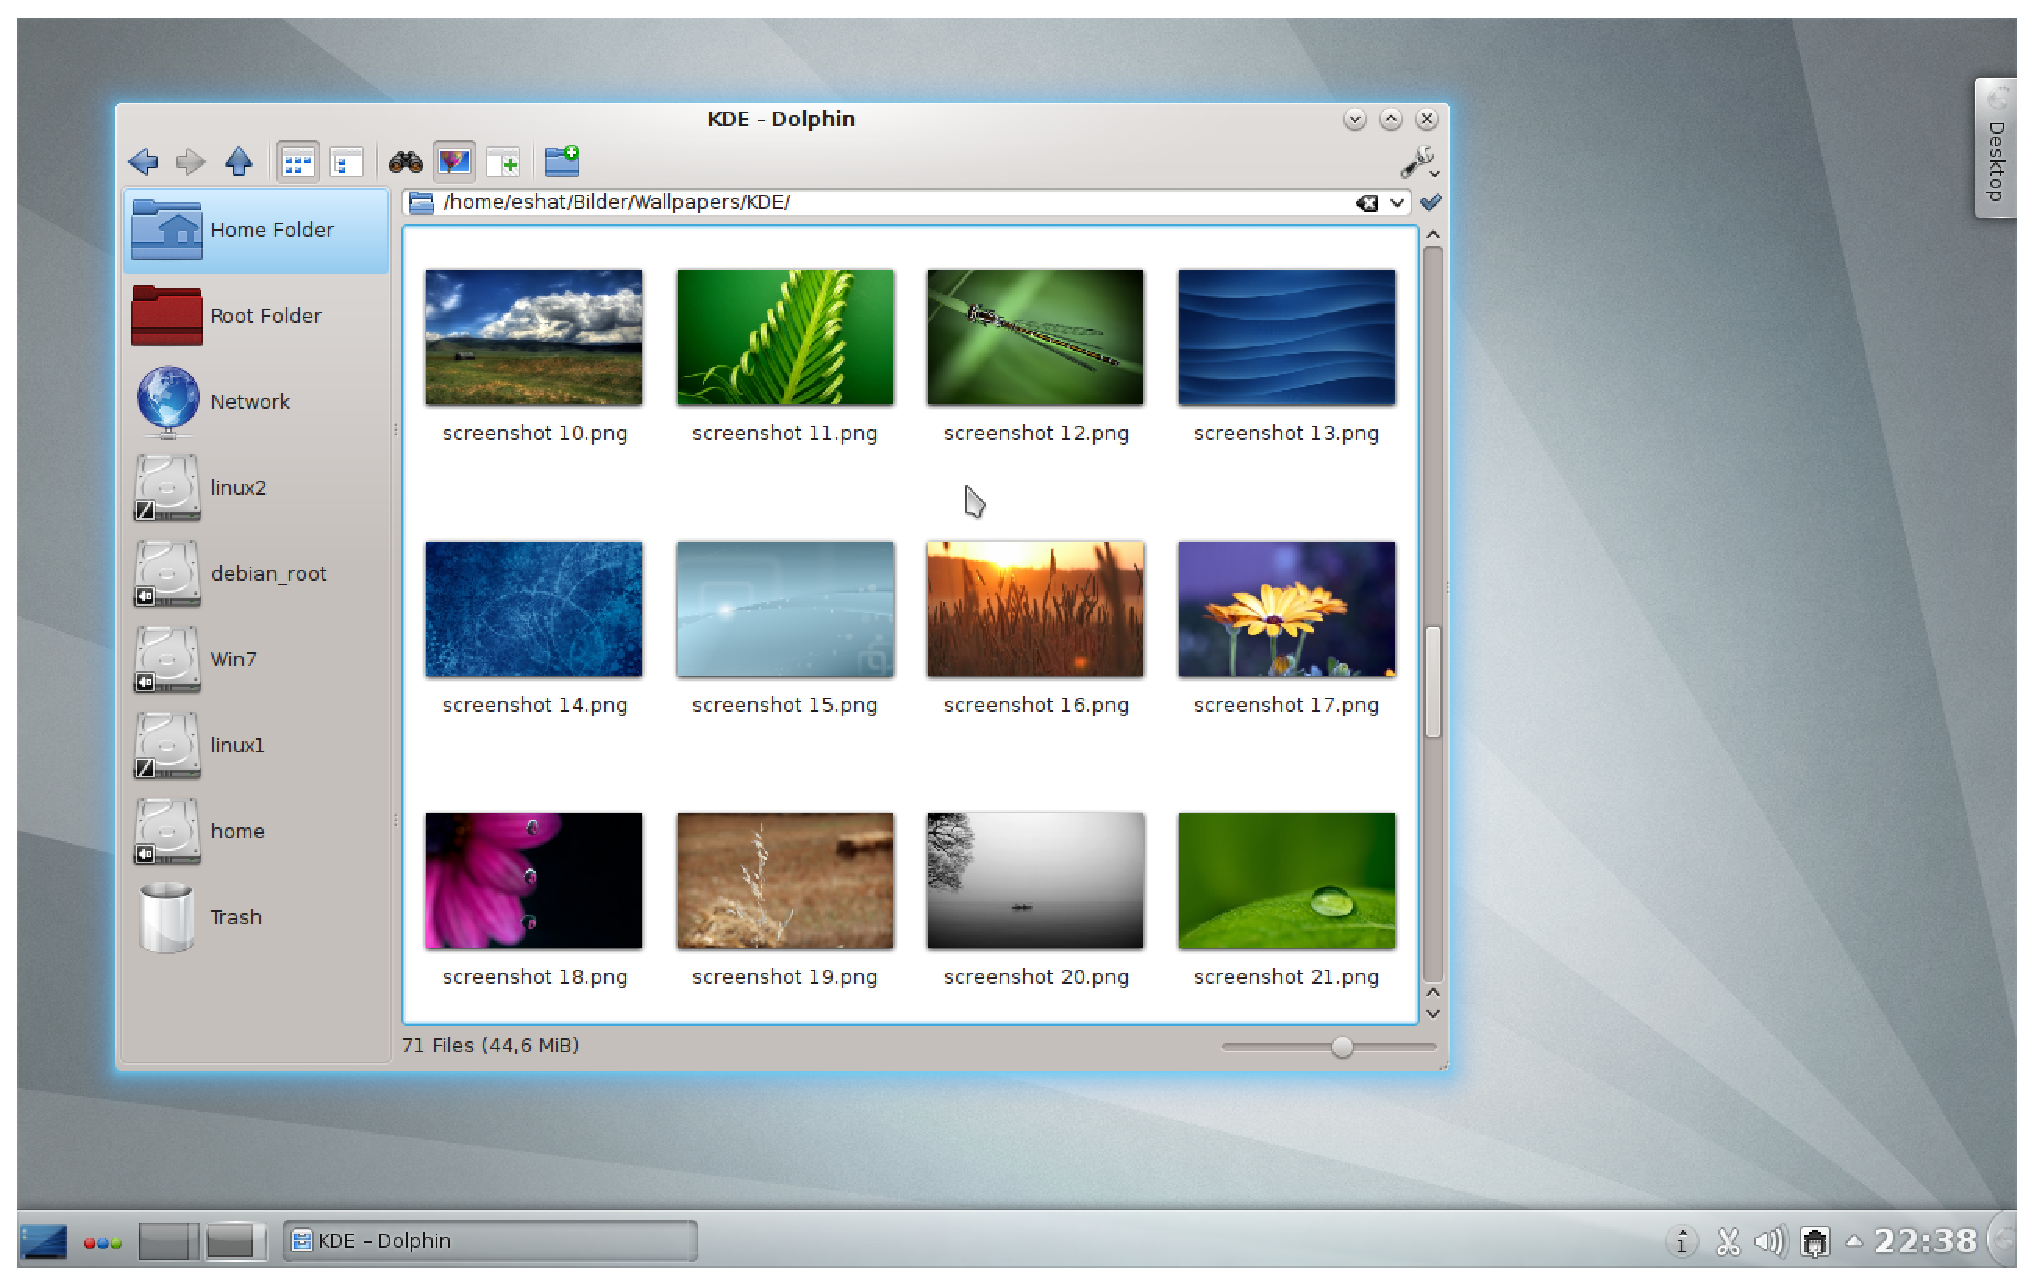
\includegraphics[scale=0.38]{base/Software/KDE1.eps}

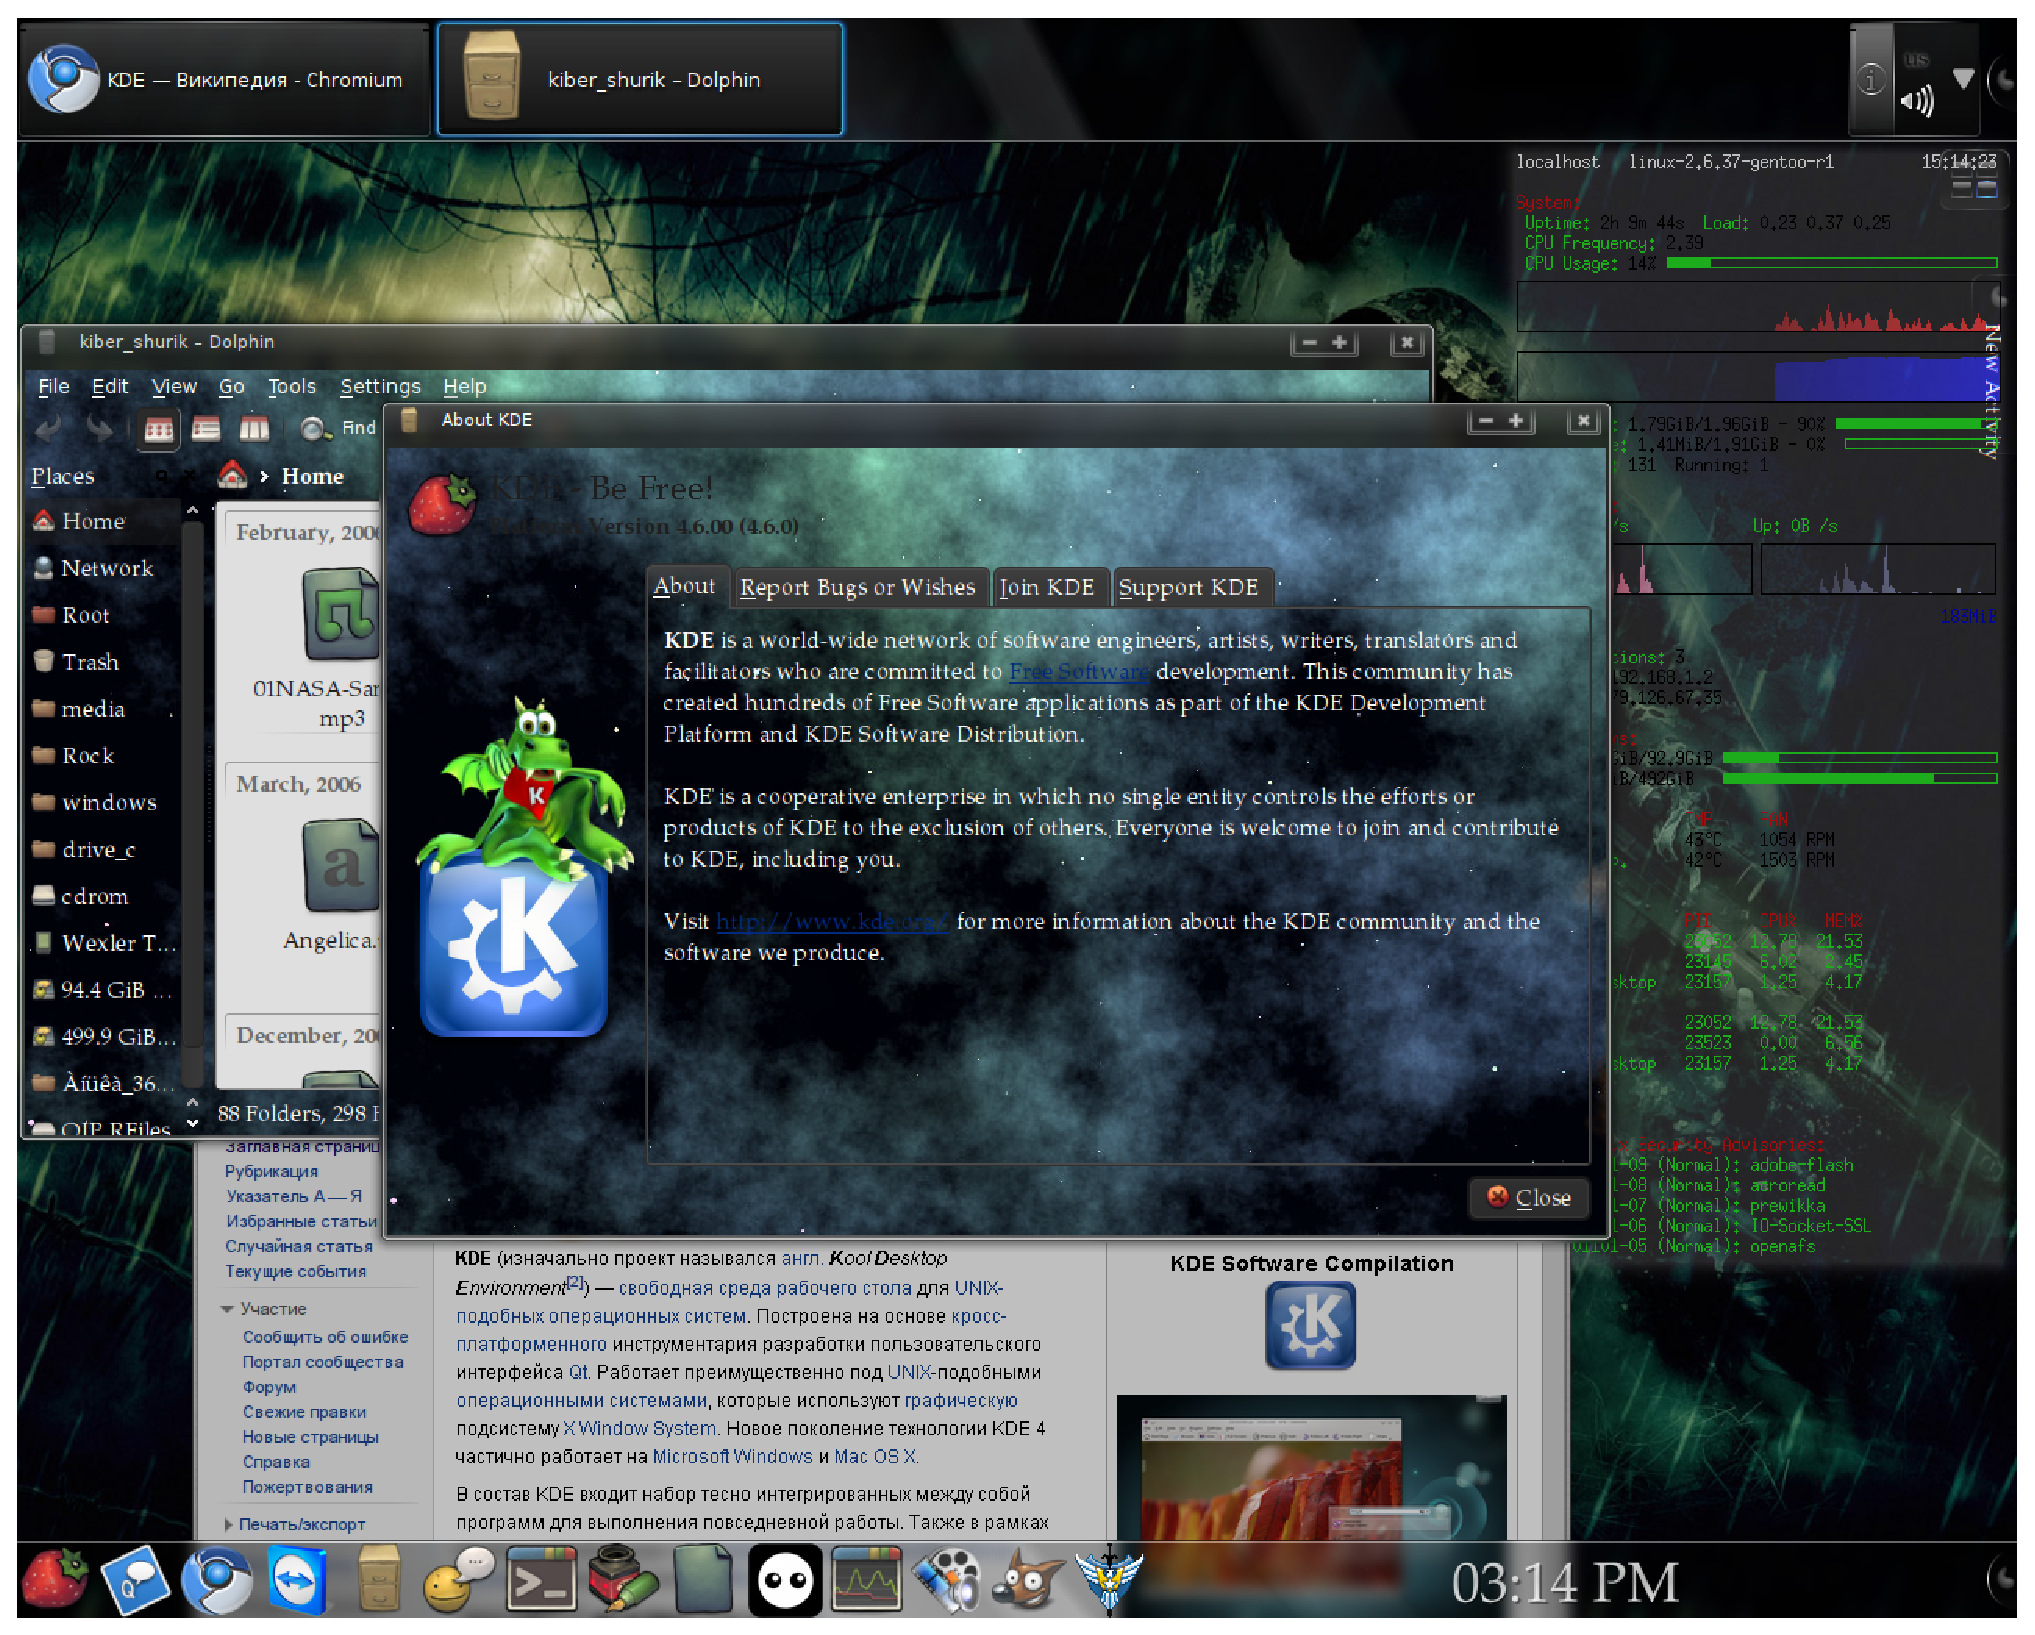
\includegraphics[scale=0.38]{base/Software/KDE2.eps}
\subsection{GNOME}
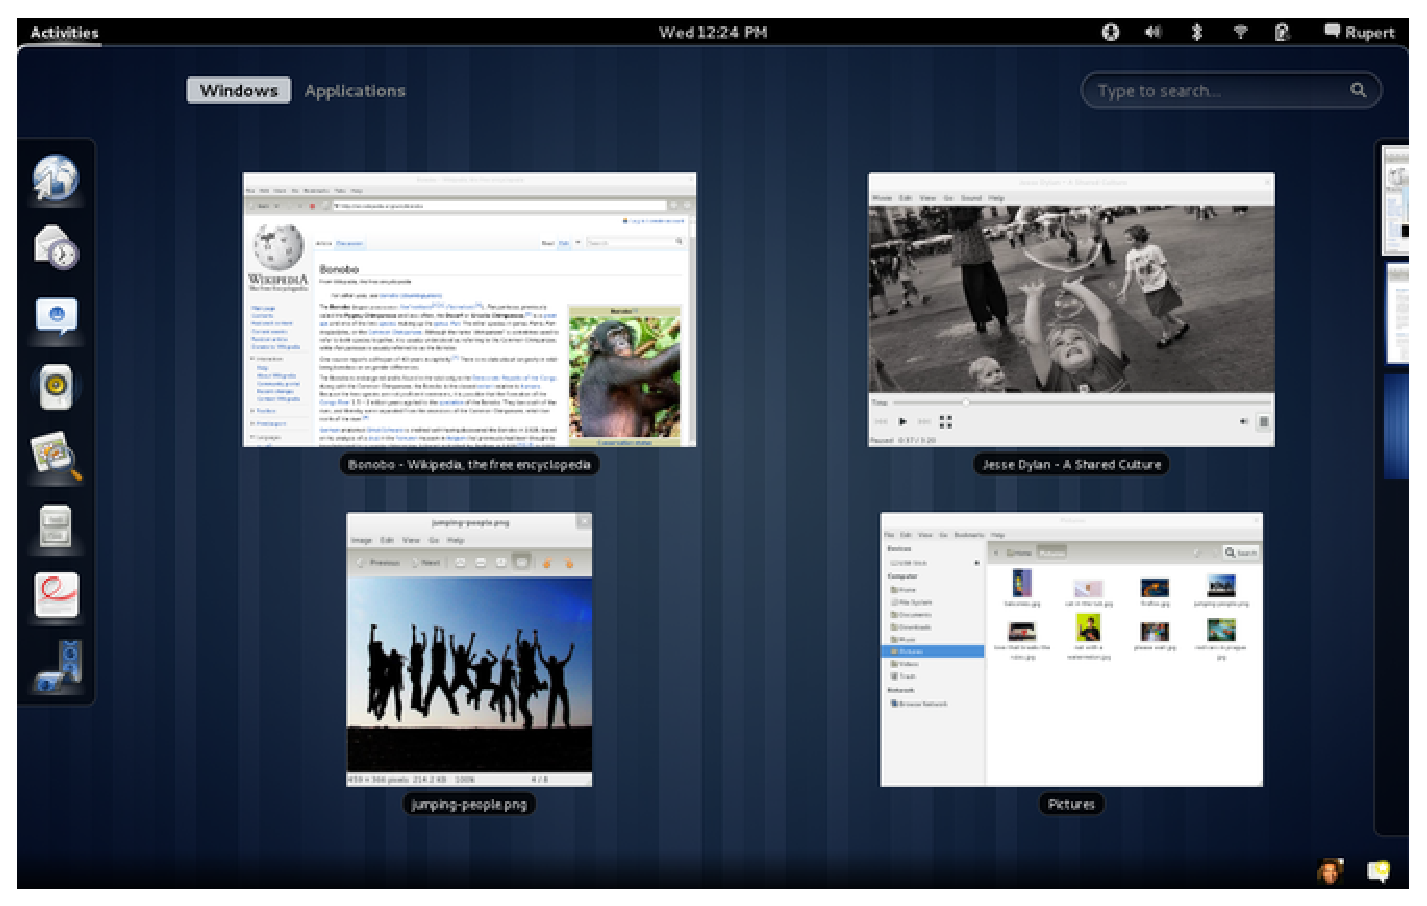
\includegraphics[scale=0.5]{base/Software/Gnome.eps}
\subsection{XFCE}
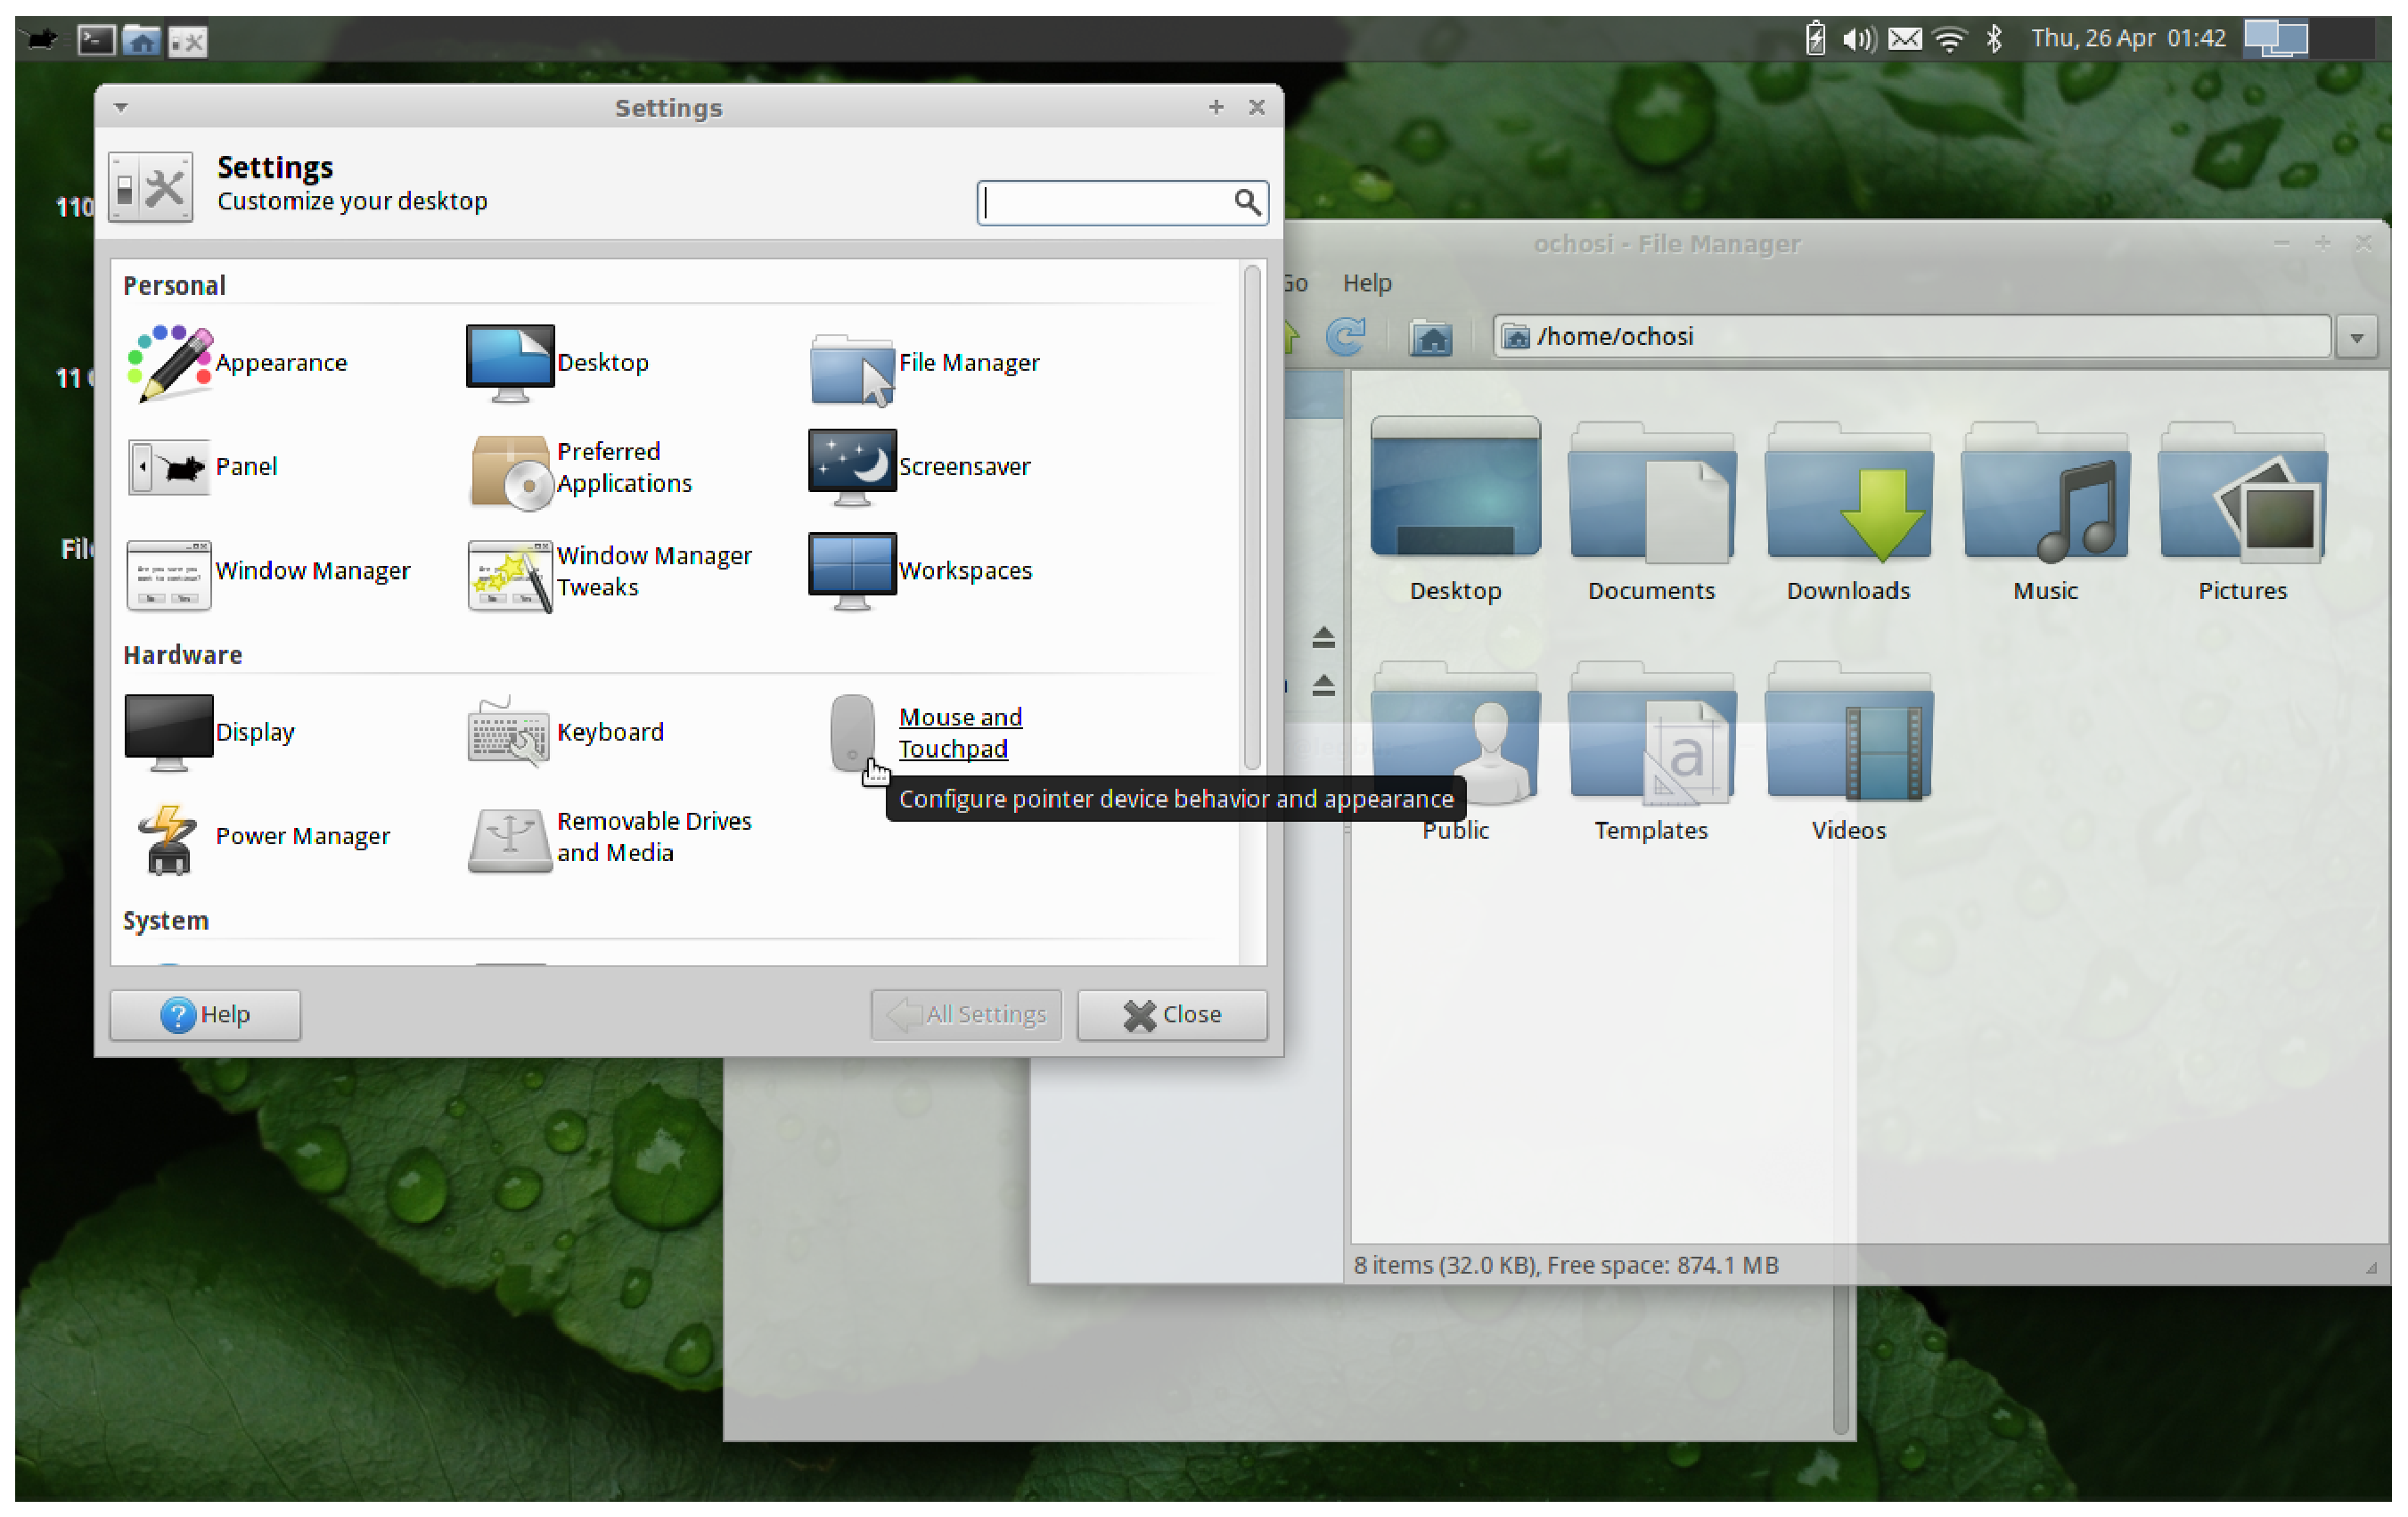
\includegraphics[scale=0.28]{base/Software/XFCE.eps}
\subsection{Unity}
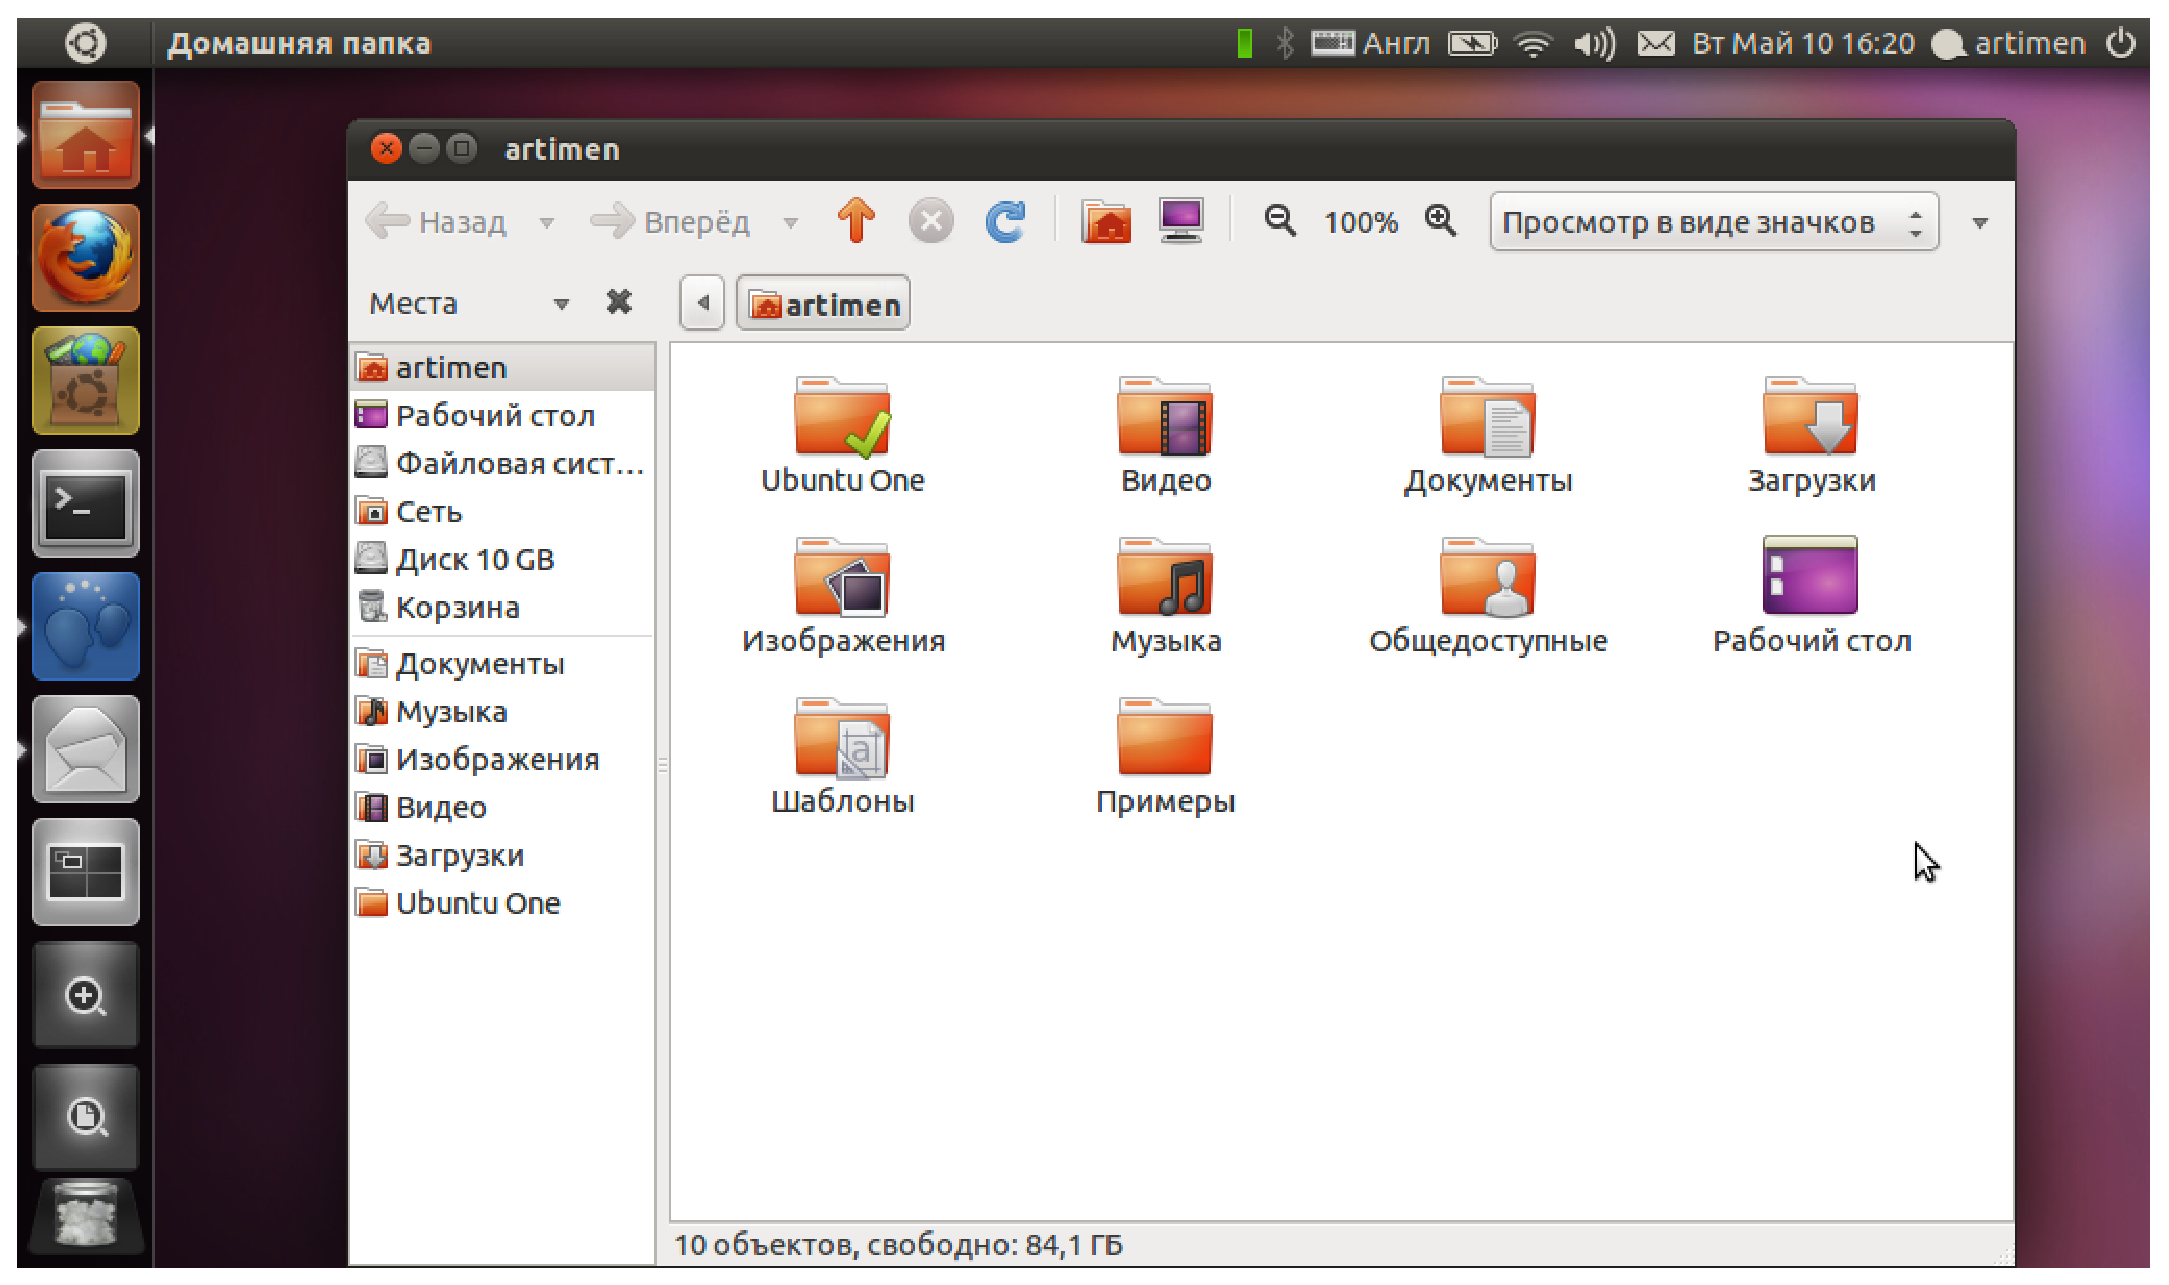
\includegraphics[scale=0.35]{base/Software/Unity.eps}
\subsection{Luna}
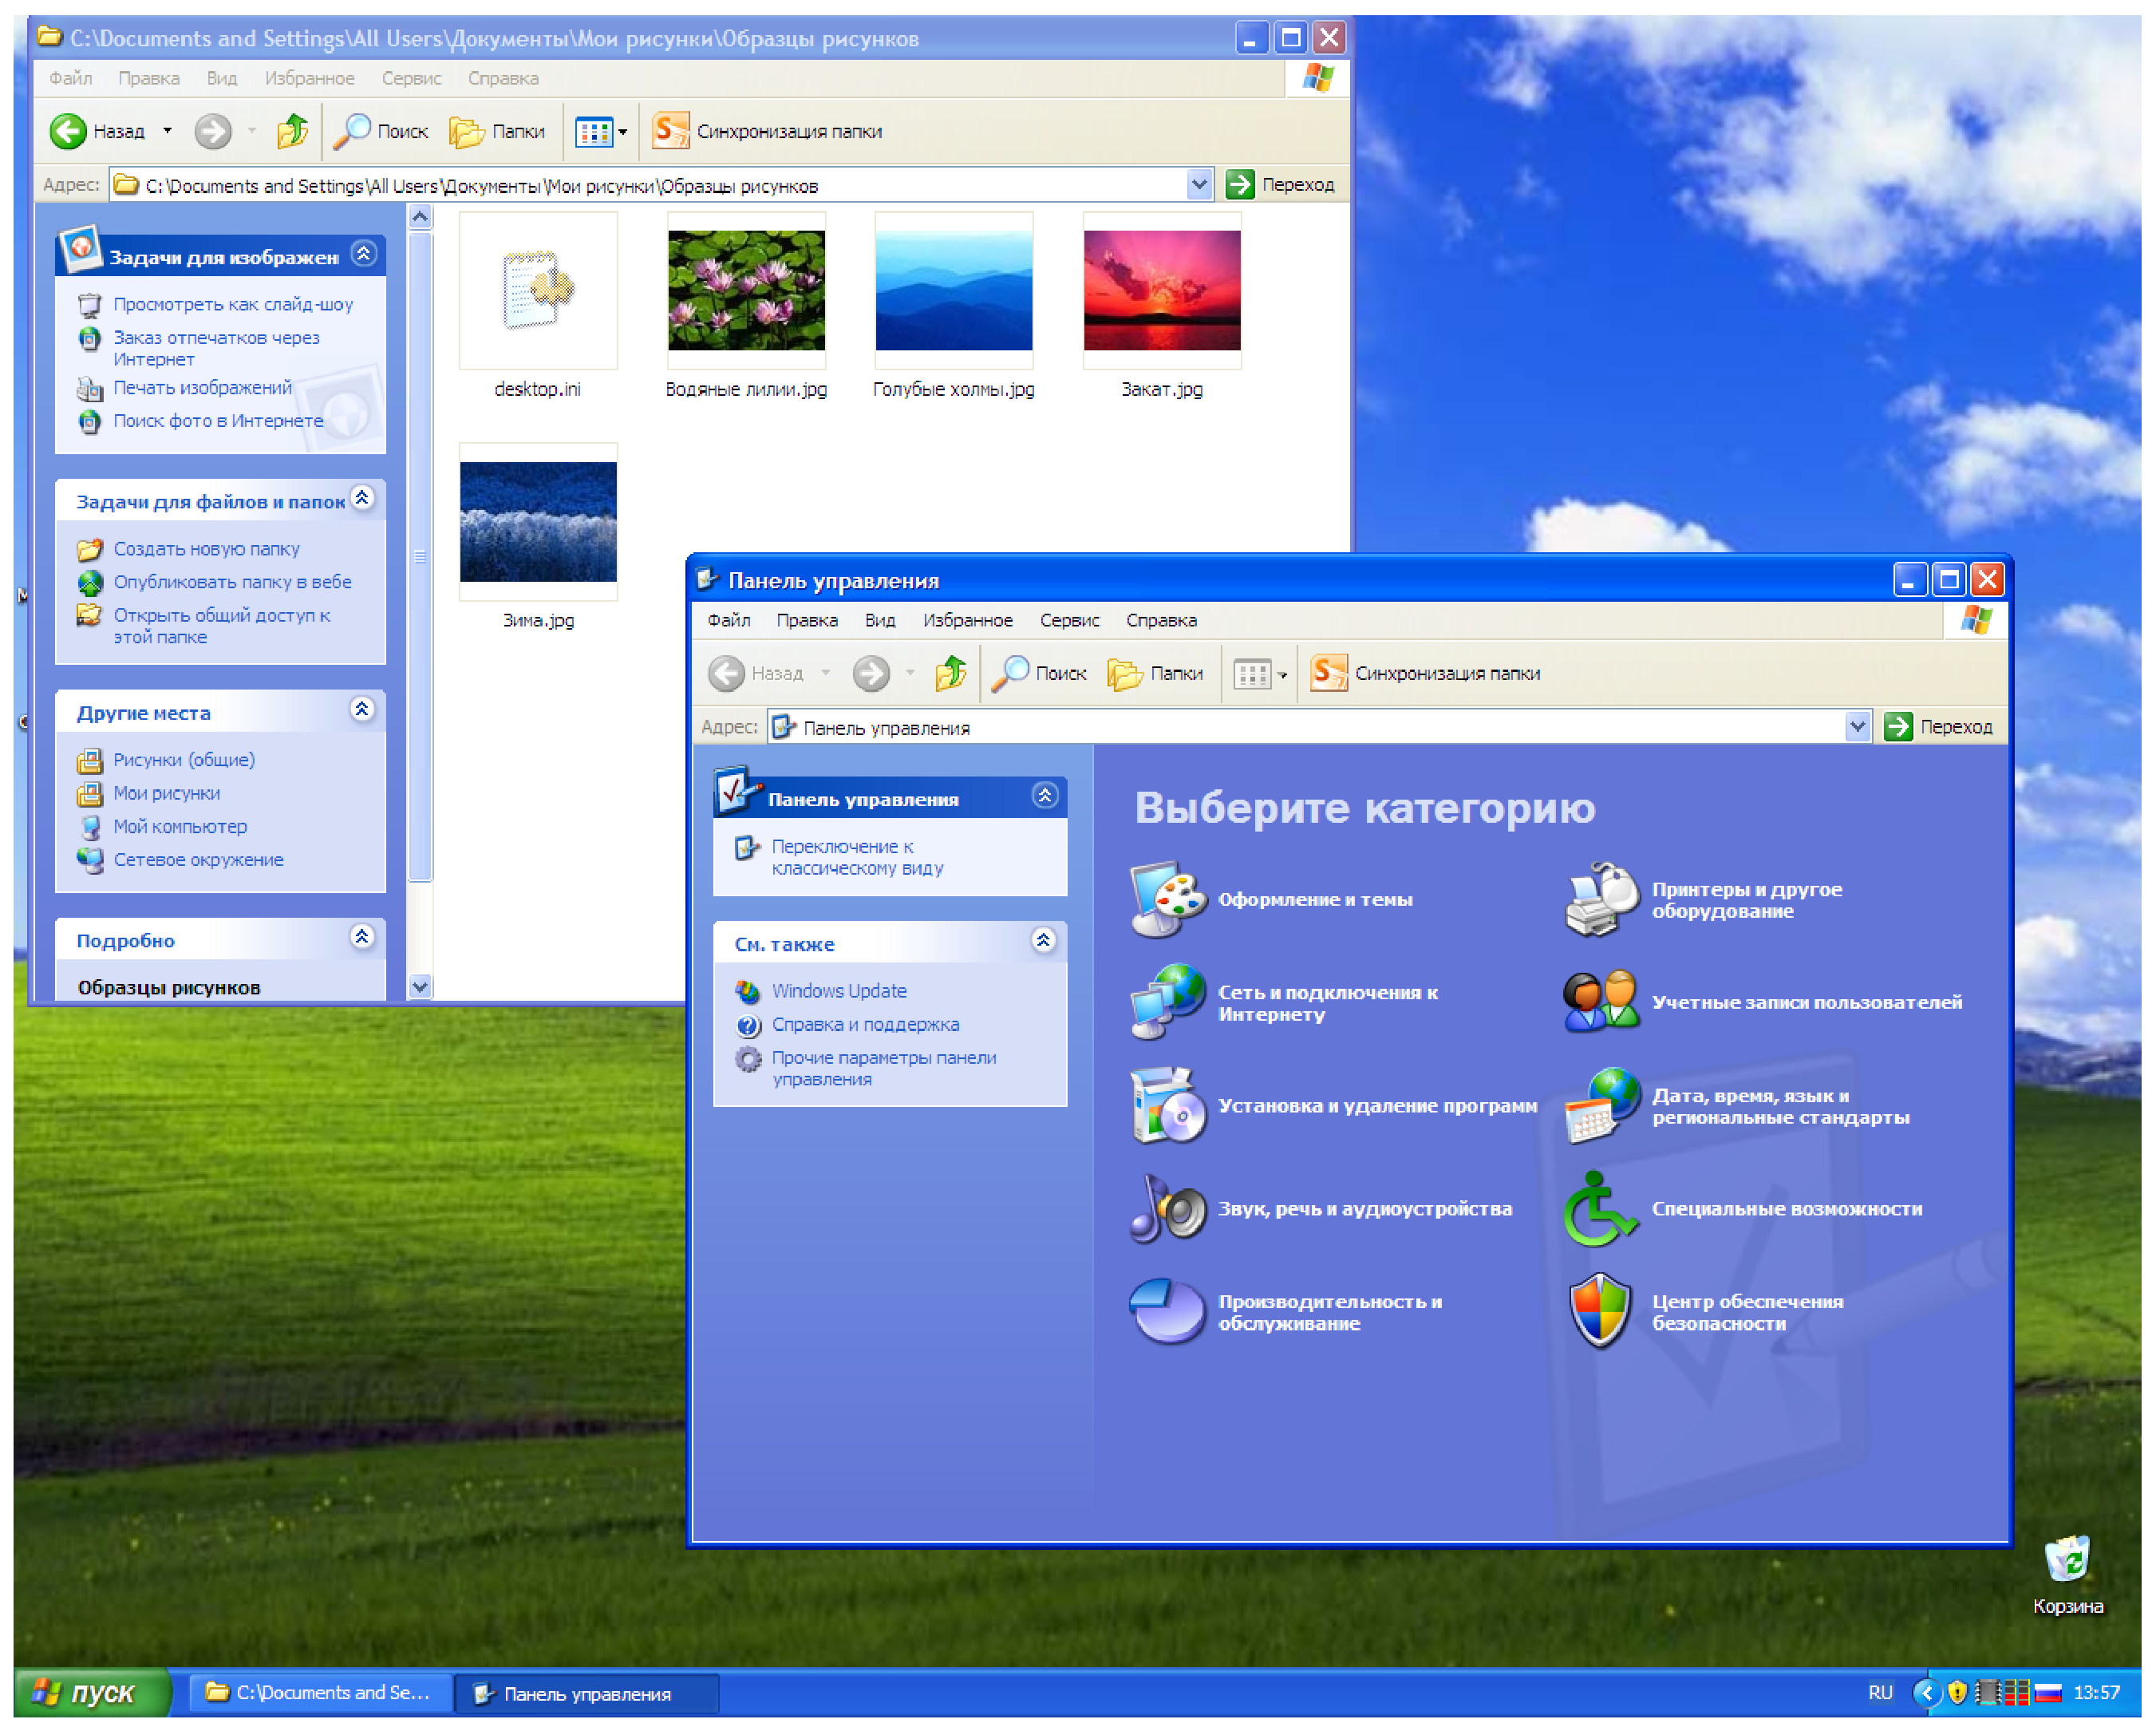
\includegraphics[scale=0.28]{base/Software/Luna.eps}
\subsection{Aero}
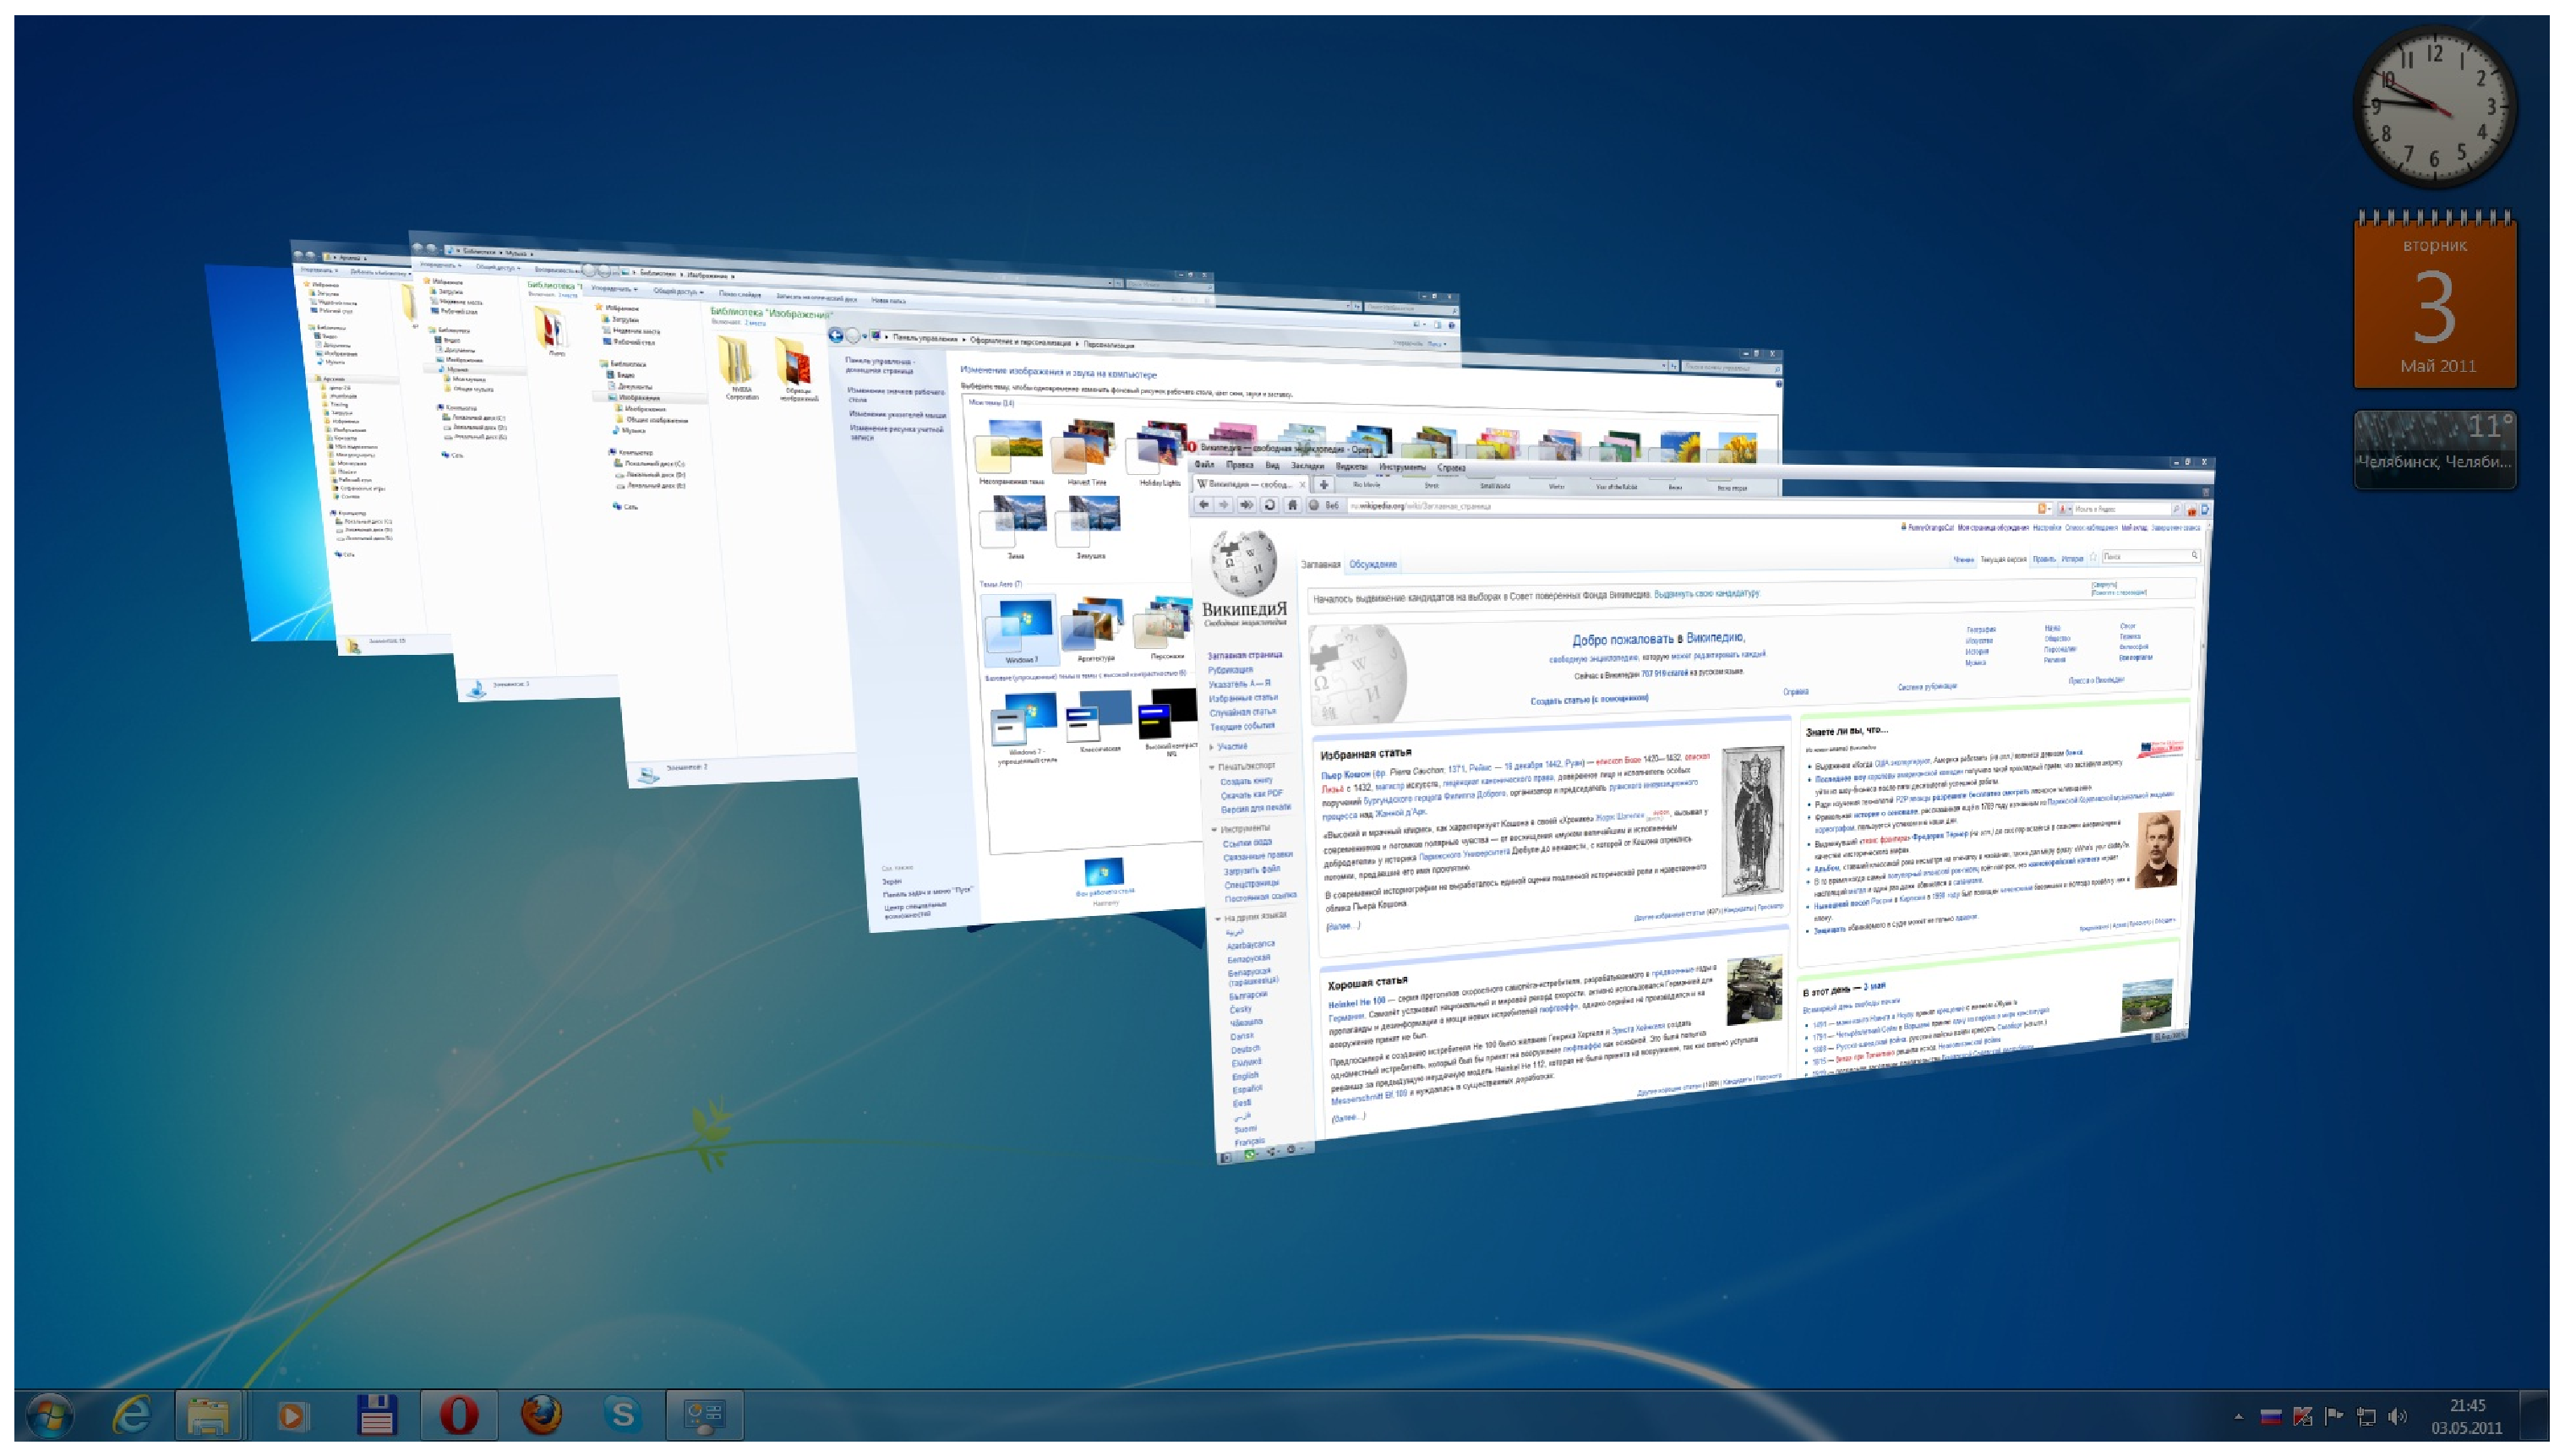
\includegraphics[scale=0.25]{base/Software/Aero}
\subsection{Aqua}
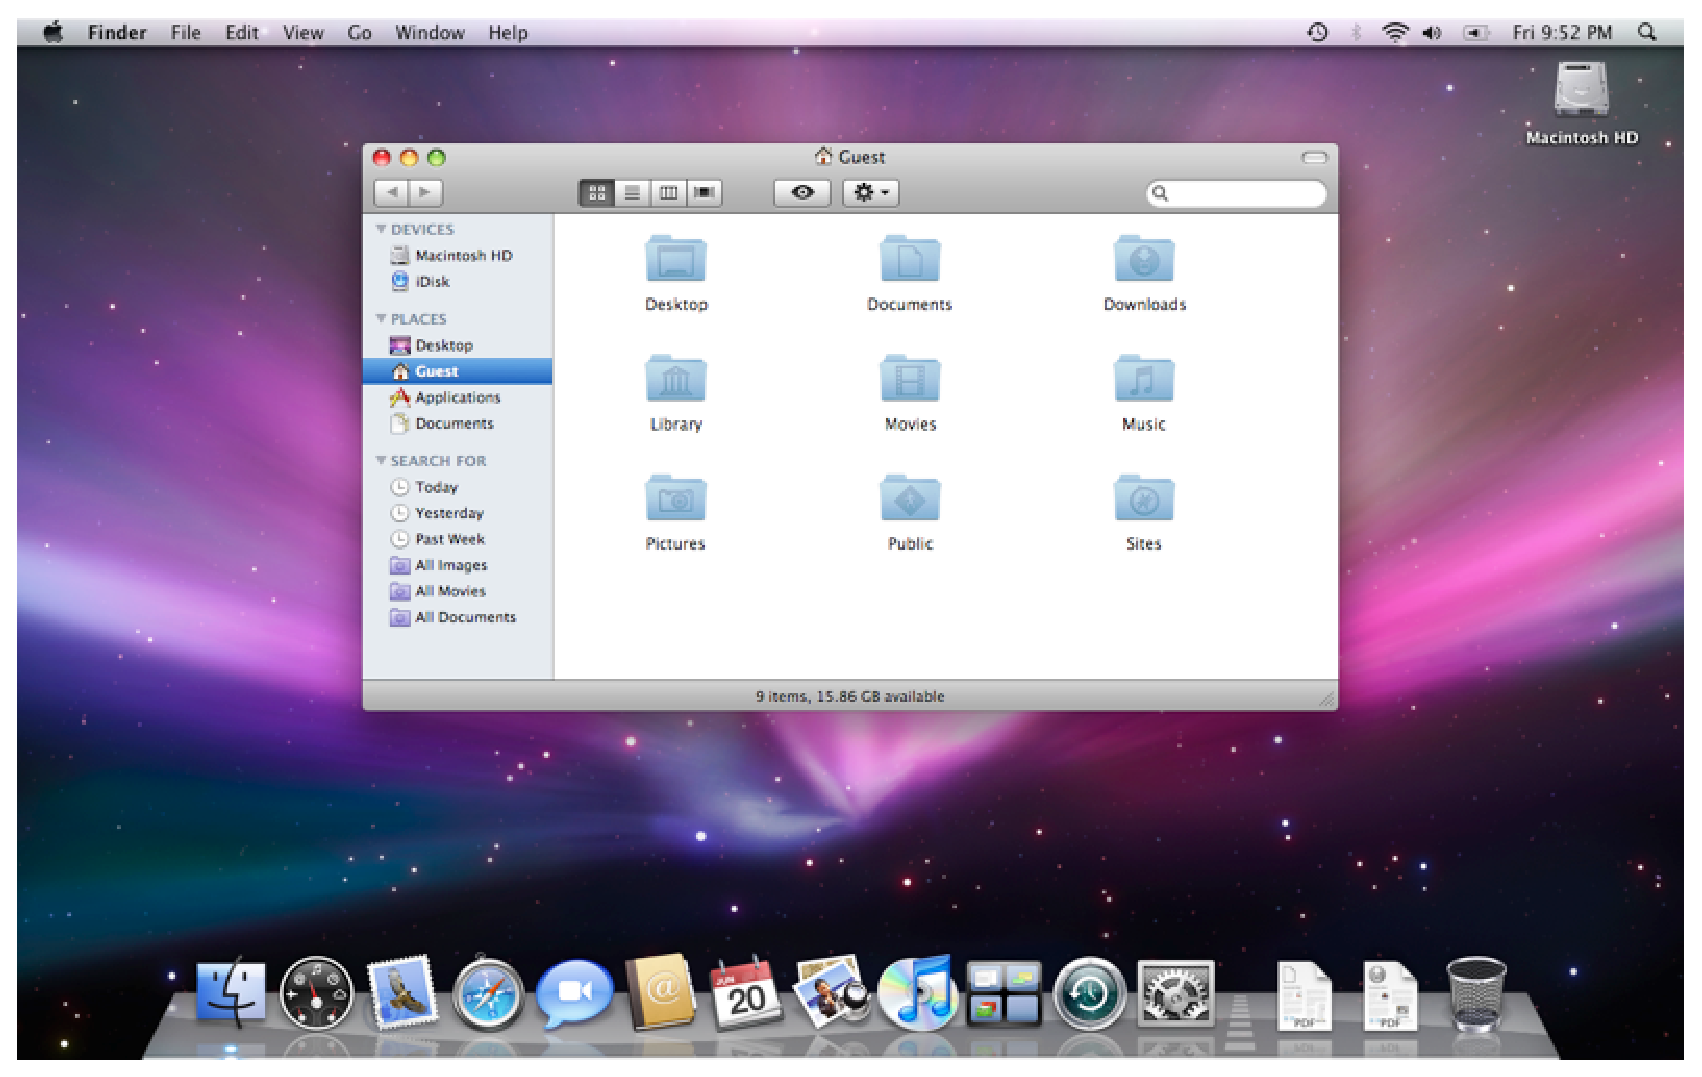
\includegraphics[scale=0.4]{base/Software/Aqua}
\subsection{Другие}

\section{Менеджеры окон}\label{base:software:wm}
\subsection{Задачи}\label{base:software:wm:tasks}
\subsection{Типы}\label{base:software:wm:types}
\subsubsection{Композитные}\label{base:software:wm:types:composite}
\subsubsection{Плавающие}\label{base:software:wm:types:float}
\subsubsection{Тайловые}\label{base:software:wm:types:tile}
\subsubsection{Динамические}\label{base:software:wm:types:dinamic}
\subsection{Элементы управления}\label{base:software:wm:controls}
\subsection{Примеры}\label{base:software:wm:examples}
\section{Работа с текстом}
123
\section{Офисные пакеты}\label{base:software:office}
123
\section{Управление пакетами}\label{base:software:packages}
123

\chapter{Аппаратное обеспечение}\label{base:hardware}
\section{Компоненты}\label{base:hardware:components}
\section{BIOS}\label{base:hardware:bios}

\chapter{Работа с сетью}
%\chapter{Введение}
Введение.
\section{Тонны матана}
%\section{Топология}\label{base:networking:topology}

%\section{ПО}\label{base:networking:software}

%\section{Протоколы}\label{base:networking:protocols}

%\section{Виртуальные сети}\label{base:networking:vpn}


\chapter{Интернет}\label{base:internet}

 \part{Программирование на C/C++}\label{cxx}
\chapter{Введение}\label{cxx:introduction}

\chapter{Основы}\label{cxx:base}

\chapter{Функции}\label{cxx:functions}

\chapter{Строки}\label{cxx:strings}

\chapter{Типы}\label{cxx:types}

\chapter{Работа с файлами}\label{cxx:files}

\chapter{Системные вызовы}\label{cxx:syscalls}


 \part{Программирование на Python}

 <<<<<<< HEAD
\part{KiCAD}

Планируемый курс, должен научить слушателей разводить печатные платы в
KiCAD. В качестве устройства для примере предлагаю использовать
USB-программатор для AVR микроконтроллеров. В идеале в дальнейшем
хотелось бы добавить информациии о том как проектируются
радиоэлектронные устройства(QUCS. ngSPICE) , а также как
программировать микроконтроллеры.

Курс будет состоять из двух циклов, базовая часть и дополнительные сведенья. 
Материалы и РЭ слушатели покупают на свои собственные деньги. 

\textbf{Оценка времени по занятиям}
\begin{itemize}
\item 2 занятия базовая Eeshema (работа создание модуля)

\item 1 cvpcb -связь УГО и footprint-ов , библиотеки и поиск

\item 2 PCBnew (работа - разводка двухслойной платы, создание
  footprnt-a)

\item 1 Генерация Gerbview и травление ЛУТ-ом (а также небольшой
  ликбез по пайке и пайка)

\item 2 Schhist работа над проектами используя git(не обязательно, но
  помогает хранить большие проекты)

\item 2 Продвинутая работа в EEshema в том числе и многостраничные
  схемы

\item 2 PCBnew -продвинуто, классы проводников , автоматическая
  разводка , footprint wizard,
\end{itemize}

KiCAD был выбран тем,что обладает доработанным интерфейсом и привычен пользователям ,а главное он обладает русскоязычной документацией и русским комьюнити.

Программатор
http://easyelectronics.ru/skorostnoj-avr-usb-programmator-na-ft232rl-bez-vspomogatelnogo-kontrollera.html
 
=======
\part{KiCAD}\label{kicad}
>>>>>>> 1d1c2a792315e5dab671ff1017b469bd4cdd9194

 \bibliographystyle{unsrt}
 \nocite{UNIX}
 \nocite{Wikipedia-en}
 \nocite{Wikipedia-ru}
 \bibliography{bibliography}
\end{document}
